%==============================================================================
%  Calibration-Aware Cross-Modal Learning for Equity Direction
%  Compile with pdfLaTeX. Self-contained: standard packages only, embedded
%  bibliography, no .bib file required.
%
%  RESULTS SWITCH
%  --------------
%  \resultsreadyfalse (default) : compiles with a visible "results pending"
%     banner and placeholder result tables.
%  \resultsreadytrue            : switch on once the walk-forward sweep has run.
%     Result tables are then read from paper/tables/*.tex, emitted by
%     finsent/eval/report.py, each carrying a provenance footnote (git sha,
%     config hash, data hash, seed list).
%
%  No number in this document is typed by hand. See SPEC.md section 6.
%==============================================================================
\documentclass[11pt,a4paper]{article}

\usepackage[utf8]{inputenc}
\usepackage[T1]{fontenc}
\usepackage[english]{babel}
\usepackage{amsmath,amssymb,amsthm}
\usepackage{booktabs}
\usepackage{array}
\usepackage{graphicx}
\usepackage{xcolor}
\usepackage{geometry}
\usepackage{caption}
\usepackage{enumitem}
\usepackage{tikz}
\usetikzlibrary{arrows.meta,positioning,fit,calc}
\usepackage[colorlinks=true,linkcolor=blue!55!black,
            citecolor=blue!55!black,urlcolor=blue!55!black]{hyperref}

\geometry{margin=2.6cm}
\captionsetup{font=small,labelfont=bf}

%--------------------------------------------------------------- num helper --
% Lightweight stand-in for siunitx \num so the file needs no extra package.
\newcommand{\num}[1]{#1}

%------------------------------------------------------------------ switches --
% ---------------------------------------------------------------------------
% Numbers quoted in running text are generated, not typed. experiments/03_make_paper.py
% writes tables/keynumbers.tex; the fallbacks below are deliberately ugly so that a
% missing or stale file is impossible to overlook in a compiled PDF.
\providecommand{\kwNames}{\textbf{??}}
\providecommand{\kwTickerDays}{\textbf{??}}
\providecommand{\kwSessions}{\textbf{??}}
\providecommand{\kwYearStart}{\textbf{??}}
\providecommand{\kwYearEnd}{\textbf{??}}
\providecommand{\kwESSFactor}{\textbf{??}}
\providecommand{\kwTests}{\textbf{??}}
\providecommand{\kwPrimaryIC}{\textbf{??}}
\providecommand{\kwPrimaryICt}{\textbf{??}}
\providecommand{\kwCovAFive}{\textbf{??}}
\providecommand{\kwCovAFiveSet}{\textbf{??}}
\providecommand{\kwCovAFiveSingle}{\textbf{??}}
\providecommand{\kwCovATen}{\textbf{??}}
\providecommand{\kwCovATenSet}{\textbf{??}}
\providecommand{\kwCovATenSingle}{\textbf{??}}
\providecommand{\kwCovATwenty}{\textbf{??}}
\providecommand{\kwCovATwentySet}{\textbf{??}}
\providecommand{\kwCovATwentySingle}{\textbf{??}}
\providecommand{\kwUngatedSharpe}{\textbf{??}}
\providecommand{\kwGateNamesHeld}{\textbf{??}}
\providecommand{\kwGateAlpha}{\textbf{??}}
\IfFileExists{tables/keynumbers.tex}{\input{tables/keynumbers.tex}}{}

\newif\ifresultsready
\resultsreadyfalse          % <--- set to \resultsreadytrue after the sweep

\newcommand{\pending}[1]{%
  \begin{center}
  \fcolorbox{red!55!black}{red!4}{%
    \parbox{0.92\linewidth}{\small\textbf{Results pending.} #1}}
  \end{center}}

% Load an auto-generated table if report.py has produced it; otherwise show a
% placeholder. This is the mechanism that makes hand-typed numbers impossible.
\newcommand{\resulttable}[3]{%
  \IfFileExists{tables/#1.tex}{\input{tables/#1.tex}}{%
    \begin{table}[t]\centering
      \caption{#2}\label{tab:#1}
      \fbox{\parbox{0.86\linewidth}{\small
        \texttt{[#1 not yet generated]}\\[3pt]
        #3\\[3pt]
        \texttt{Produce with: make reproduce}}}
    \end{table}}}

%------------------------------------------------------------------- theorems --
\theoremstyle{plain}
\newtheorem{proposition}{Proposition}
\newtheorem{corollary}[proposition]{Corollary}
\theoremstyle{definition}
\newtheorem{definition}{Definition}
\theoremstyle{remark}
\newtheorem{remark}{Remark}

%--------------------------------------------------------------------- macros --
\newcommand{\R}{\mathbb{R}}
\newcommand{\E}{\mathbb{E}}
\newcommand{\Prob}{\mathbb{P}}
\newcommand{\muhat}{\hat{\mu}}
\newcommand{\sigmahat}{\hat{\sigma}}
\newcommand{\fstar}{f^{\star}}
\newcommand{\LN}{\mathrm{LN}}
\newcommand{\ECE}{\mathrm{ECE}}
\newcommand{\Down}{\textsc{down}}
\newcommand{\Neutral}{\textsc{neutral}}
\newcommand{\Up}{\textsc{up}}

\title{\bfseries Calibration Is the Binding Constraint on Position
Sizing:\\[2pt] Growth-Optimal Decisions, Conformal Abstention, and an\\
Honest Walk-Forward Protocol for Equity Direction}

\author{%
  \textit{Author One}\thanks{Corresponding author. Replace this block before
  submission.}\quad \textit{Author Two}\quad \textit{Author Three}\\[2pt]
  \small Department of Computer Science, Institution\\
  \small \texttt{author@institution.edu}}

\date{\today}

\begin{document}
\maketitle

%==============================================================================
\begin{abstract}
\noindent
Directional forecasts of equity returns are almost universally evaluated by
accuracy, yet accuracy is not the quantity that determines the economic outcome
once a forecast becomes a position. We argue, prove and measure that
\emph{calibration} --- the agreement between stated probability and realised
frequency --- is the binding constraint on growth-optimal position sizing, and
we quantify what miscalibration costs. We first show analytically that the
expected log-growth penalty incurred by a miscalibrated forecast equals one
half the squared standardised error of the conditional mean, and that
underestimating the conditional variance by a factor of two eliminates the
entire growth advantage of a genuinely profitable signal. We then present
\textsc{FinSentNet-C}, a compact cross-modal model (\num{448{,}453} trainable
parameters) that fuses cached financial-news embeddings with a causal price
encoder through a single gated cross-attention block with modality dropout, and
that jointly predicts direction, conditional mean and conditional variance
under a differentiable calibration objective. Predictions are calibrated per
fold by guarded vector scaling and wrapped in adaptive conformal prediction
sets, so that a position is taken only when the model's uncertainty set is a
singleton. The evaluation protocol is point-in-time, purged and embargoed,
refitted semi-annually and multi-seed; every reported figure carries a
confidence interval, a Diebold--Mariano test against each baseline, a Deflated
Sharpe Ratio and a Probability of Backtest Overfitting computed against a
declared trial budget. Beyond the model we report two methodological failure
modes, measured on controlled data and easily missed in practice: a
one-session execution-lag defect that inflates a trailing-return feature's
cross-sectional rank information coefficient from \num{0.004} to \num{0.108} on
driftless data while remaining invisible to any train/test splitter, and a
regime in which unguarded post-hoc calibration reduces validation calibration
error from \num{0.020} to \num{0.004} while \emph{raising} held-out error from
\num{0.003} to \num{0.056}.
On a point-in-time universe of \kwNames{} liquid US names over
\kwYearStart--\kwYearEnd{} (\kwTickerDays{} ticker-days), the protocol returns
a null. No model we test, including \textsc{FinSentNet-C}, produces a
\emph{positive} rank information coefficient distinguishable from zero (\kwPrimaryIC{},
Newey--West $t=\kwPrimaryICt$), and none clears realistic trading costs. The
decision layer, however, behaves exactly as the theory requires. Conformal
coverage is empirically exact --- \kwCovAFive{} against a nominal \num{0.95}
and \kwCovATen{} against a nominal \num{0.90} --- and precisely because a model
without an edge cannot produce a singleton prediction set at those levels
(mean set size \kwCovATenSet{} of three possible classes), the abstention gate
declines every name and takes no position at all. It is the only one of the
four sizing rules we compare that does not lose money, and it dominates by
refusing to bet. We regard this as the paper's central empirical finding rather
than a disappointing one: a decision layer earns its place by what it declines,
and a protocol earns its place by being willing to return a null.
\end{abstract}

\noindent\textbf{Keywords:} probability calibration; conformal prediction;
growth-optimal sizing; cross-modal fusion; financial machine learning;
backtest overfitting.

\ifresultsready\else
\pending{This manuscript compiles in \emph{draft} mode. The walk-forward sweep
specified in Section~\ref{sec:protocol} has not been executed, so
Section~\ref{sec:results} contains placeholders rather than numbers. Set
\texttt{\textbackslash resultsreadytrue} in the preamble once
\texttt{finsent/eval/report.py} has emitted \texttt{paper/tables/*.tex}. Every
result table is read from that directory and carries its own provenance
footnote; no number in this document is entered by hand. The figures in
Section~\ref{sec:validation} are measurements on \emph{controlled synthetic
data} whose ground truth is known, and are labelled as such throughout.}
\fi

%==============================================================================
\section{Introduction}
\label{sec:intro}

A forecast becomes useful only when it becomes a position, and the map from one
to the other is not neutral. Two models with identical directional accuracy can
produce very different terminal wealth, because the rule converting a
probability into a bet size is convex in that probability's error. The
literature on machine learning for equity returns has concentrated almost
entirely on the first half of this sentence --- accuracy, macro-$F_1$,
occasionally an information coefficient --- and has treated sizing as an
implementation detail appended once the modelling is finished.

This paper takes the opposite view. At the signal-to-noise ratio available in
daily equity data, the marginal value of another point of accuracy is small and
statistically hard to establish, whereas the marginal value of a correctly
calibrated probability is large, provable and measurable with far greater
precision. The reason is arithmetic. Calibration error is estimated over
hundreds of thousands of individual predictions; a Sharpe ratio is estimated
over a few thousand daily portfolio returns. The standard error of the former
is roughly an order of magnitude smaller. A research programme that stakes its
claim on calibration is therefore \emph{testable} at effect sizes where a claim
staked on alpha is not.

\paragraph{The claim.}
Calibrated probability, not raw accuracy, determines whether a directional
equity signal survives position sizing. Concretely: (i) cross-modal gating
improves calibration more than it improves accuracy; and (ii) calibration-aware
growth-optimal sizing converts a small, statistically fragile predictive edge
into a materially better risk-adjusted outcome than the \emph{same} predictions
sized by uncalibrated softmax confidence. The second is the headline experiment,
and it is constructed so that predictions are held fixed and only the sizing
rule varies. Because the comparison is paired, most common variance cancels and
the test retains power at edge sizes where an unpaired strategy comparison
would be hopeless.

\paragraph{Why this is not merely an engineering point.}
Section~\ref{sec:decision} makes the claim quantitative. For a position of
fraction $f$ in an asset with conditional mean $\mu$ and variance $\sigma^2$,
expected log-growth is $G(f)=f\mu-\tfrac12 f^2\sigma^2$, maximised at
$\fstar=\mu/\sigma^2$ with $G(\fstar)=\mathrm{SR}^2/2$: the maximum achievable
log-growth rate is half the squared Sharpe ratio. We show that a wrong mean
costs exactly $(\mu-\muhat)^2/(2\sigma^2)$ --- one half the squared
standardised forecast error --- and that a wrong variance costs a fraction
$(1-u)^2$ of the optimum, with $u=\sigma^2/\sigmahat^2$. The second result
carries a corollary worth stating in an introduction: underestimating
conditional variance by a factor of two drives expected log-growth to
\emph{exactly zero} on a signal that is genuinely profitable. Since
overconfidence \emph{is} variance underestimation, this is the mechanism by
which a confident model loses to a flat one.

\paragraph{Evidence discipline.}
Equity return prediction is a field in which reported results routinely fail to
replicate, and the causes are catalogued: survivorship in the universe,
overlapping labels, unpurged splits, unstated execution conventions, and
selection over a large undeclared trial budget. We adopt the corresponding
controls throughout and --- because a control is only as good as its
verification --- we additionally report, in Section~\ref{sec:validation}, what
happens when two of them are removed. Both failure modes were found by
instrumentation rather than inspection, both would have produced a
publishable-looking number, and neither is detectable by any train/test
splitter.

\paragraph{Contributions.}
\begin{enumerate}[leftmargin=1.6em,itemsep=2pt]
\item \textbf{A theory of what miscalibration costs.} Three propositions
  relating expected log-growth loss to mean-forecast error, variance-forecast
  error and expected calibration error, each verified numerically against
  simulated compounding (Section~\ref{sec:decision}).
\item \textbf{A compact gated cross-modal architecture} with modality dropout,
  at \num{448{,}453} trainable parameters against roughly \num{220{,}000}
  effectively independent training samples (Section~\ref{sec:model}). We are
  explicit that this contribution is a \emph{specification}: the corpus
  available to us cannot support a point-in-time text claim, so every number we
  report comes from the model run in a forced price-only state, and the fusion
  pathway is offered for replication rather than demonstrated.
\item \textbf{Calibration-aware training and conformal abstention}: a
  differentiable calibration objective, guarded per-fold post-hoc calibration in
  which the identity map competes as a genuine candidate, and adaptive conformal
  sets that gate trading on singleton uncertainty
  (Sections~\ref{sec:objective}--\ref{sec:calibration}).
\item \textbf{A leakage-controlled evaluation protocol}, pre-specified in
  Section~\ref{sec:protocol}, with the measured demonstration in
  Section~\ref{sec:validation} that its components are load-bearing rather than
  ceremonial.
\item \textbf{A null result, reported as one.} On \kwTickerDays{} ticker-days
  no model we test produces a positive rank information coefficient that
  survives a Newey--West standard error, and none clears realistic costs. We
  report this rather than searching for the configuration that would not have
  produced it. Along the way the protocol caught three defects in our own
  pipeline, each of which would have produced a plausible-looking result: an
  execution-lag leak worth an apparent rank IC of \num{0.108} on driftless
  data, an unguarded post-hoc calibration step that improved validation
  calibration while degrading held-out calibration by an order of magnitude,
  and a position-sizing rule that saturated every weight at its cap because it
  sized the level of the conditional mean rather than its cross-sectional
  deviation.
\item \textbf{A released, tested implementation.} The data, evaluation,
  calibration, conformal and decision layers depend only on
  NumPy/pandas/SciPy, so the paper's statistical claims reproduce without a
  deep-learning installation; \kwTests{} test functions accompany the code, and
  every table and every number quoted in the text is emitted by the release
  rather than transcribed into it.
\end{enumerate}

\paragraph{Relation to prior work by the authors.}
This paper supersedes an earlier design by the same authors that used a deeper
text stack, a fixed-threshold label, a single chronological holdout and a
barrier-odds Kelly rule. Appendix~\ref{app:supersede} lists the specification
conflicts that reconciliation resolved, since several changed the meaning of
reported quantities rather than merely their values.

%==============================================================================
\section{Related Work}
\label{sec:related}

\paragraph{Machine learning in empirical asset pricing.}
The modern reference point is \citet{gu2020empirical}, whose comparison of
regularised linear models, trees and neural networks over a large panel
establishes both the achievable signal level and the evaluation conventions the
field has converged on. \citet{kellyxiu2023} survey it; \citet{chen2024deep}
extend it with deep conditional asset-pricing models, and
\citet{jiang2023reimagining} show that convolutional encoders over price charts
recover recognisable technical structure. A consistent finding is that flexible
models do not dominate regularised linear ones by wide margins at this
signal-to-noise ratio, which is the empirical basis for the capacity argument
of Section~\ref{sec:capacity}. \citet{fischer2018deep} give the recurrent
benchmark most directly comparable to a daily directional model.

\paragraph{Text and returns.}
\citet{tetlock2007giving} established that a simple count of negative words in
a widely read column predicts returns and volume, and
\citet{loughran2011liability} showed that general-purpose sentiment lexicons
misread financial language. Transformer encoders adapted to financial corpora
followed \citep{araci2019finbert,yang2020finbert,huang2023finbert}; at least
three distinct models are called FinBERT, and we state our checkpoint
explicitly in Appendix~\ref{app:hyper}. \citet{ke2019predicting} extract
return-predictive content with a supervised topic model, and
\citet{lopezlira2023chatgpt} report that instruction-tuned language models score
headlines competitively, which motivates our LLM-scored-sentiment baseline.
\citet{dong2024fnspid} and \citet{zhou2021trade} provide timestamped,
ticker-linked corpora that make the text modality reproducible;
\citet{xu2018stocknet} remains the standard paired text--price benchmark.

\paragraph{Cross-modal fusion.}
Query--key--value interaction across modalities was formalised in
vision-and-language work \citep{lu2019vilbert,chen2020uniter}. The gating
mechanism descends more directly from gated multimodal units
\citep{arevalo2017gated}. In finance, \citet{hu2018listening} pair a news
encoder with attention over price sequences and
\citet{sawhney2021quantitative} attend between transcripts and price graphs.
Our block is deliberately shallow --- one block, four heads --- and pairs the
gate with modality dropout, which converts the fusion ablation from a
retraining exercise into an evaluation-time intervention on one set of weights.

\paragraph{Calibration and distribution-free uncertainty.}
\citet{guo2017calibration} documented the miscalibration of modern networks and
introduced temperature and vector scaling. Binned calibration error is
piecewise constant in the parameters and therefore has no useful gradient, so
training-time calibration requires a surrogate; we use the kernel statistic of
\citet{kumar2018trainable}. \citet{mukhoti2020calibrating} show that focal loss
itself alters calibration, which is why we keep it off by default and treat it
as an ablation. For set-valued prediction we use split conformal
\citep{vovk2005algorithmic,angelopoulos2021gentle} with the adaptive-set score
of \citet{romano2020classification} and the online update of
\citet{gibbs2021adaptive}, which maintains coverage under the distribution
shift that financial data reliably supplies.

\paragraph{Sizing, and evaluation under selection.}
Growth-optimal betting originates with \citet{kelly1956new}; the
continuous-outcome analogue is \citet{merton1969lifetime}, and
\citet{maclean2011kelly} collect the fractional-Kelly literature motivating
$\kappa<1$. Our propositions are, to our knowledge, the first explicit
statement in this applied literature of the log-growth penalty as a function of
\emph{calibration} error specifically. On evaluation we follow
\citet{lopezdeprado2018advances} for purging, embargoing and label uniqueness;
\citet{bailey2014deflated} for the Deflated Sharpe Ratio;
\citet{bailey2017probability} for the Probability of Backtest Overfitting;
\citet{diebold1995comparing}, \citet{white2000reality} and
\citet{hansen2005test} for predictive-accuracy and multiple-comparison tests;
and \citet{harvey2016and} for the significance threshold appropriate to a
discovered factor. Costs follow the square-root impact tradition
\citep{almgren2005direct,frazzini2018trading,novymarx2016comparative}, and
covariance estimation follows \citet{ledoit2004well}.

%==============================================================================
\section{Problem Formulation}
\label{sec:formulation}

\subsection{Universe}
Let $\mathcal{U}_t$ denote the tradeable names on session $t$. It is
constructed \emph{point-in-time}: membership on $t$ uses only information
available strictly before $t$, and delisted names simply cease to appear. Our
default construction is a liquidity screen --- top $N$ by trailing median
dollar volume, rebalanced monthly, subject to a price floor --- because it is
fully reproducible from freely available daily data and contains no forward
information. We describe it as a liquidity-screened universe rather than as an
index, which is the accurate description.

Applying a \emph{current} index membership list retroactively is the most
consequential data defect available in this setting: names leave an index
disproportionately after poor performance, so a backtest on today's members is
a backtest on companies selected for having survived. Our implementation ships
a membership diagnostic that fails when no name present on the first date is
absent by the last, since that pattern is the signature of a retroactively
applied list.

\subsection{The timestamp contract}
\label{sec:timestamps}
Decisions execute at the \emph{open}. A headline published at $\tau$ may inform
the decision executed at the open of session $t$ if and only if
\begin{equation}
\mathrm{open}(t)\;\ge\;\tau+\Delta,\qquad \Delta=24\ \text{hours},
\label{eq:lag}
\end{equation}
and returns are measured open-to-open from $\mathrm{open}(t)$ to
$\mathrm{open}(t+h)$. Table~\ref{tab:timestamps} works the rule through three
cases; the second is the one most often got wrong.

\begin{table}[t]
\centering
\caption{The timestamp contract of Equation~\eqref{eq:lag} with a 09:30
US/Eastern open. A 16:30 headline is \emph{not} usable at the next morning's
open: only 17 hours have elapsed.}
\label{tab:timestamps}
\small
\begin{tabular}{lll}
\toprule
\textbf{Publication (US/Eastern)} & \textbf{Decision open} & \textbf{Return window}\\
\midrule
Tue 09:00 (before Tuesday's open) & Wed 09:30 & Wed open $\to$ Wed$+h$ open\\
Tue 16:30 (after Tuesday's close) & Thu 09:30 & Thu open $\to$ Thu$+h$ open\\
Sat 03:00 (weekend)               & Mon 09:30 & Mon open $\to$ Mon$+h$ open\\
\bottomrule
\end{tabular}
\end{table}

\begin{remark}[Features must be lagged, not merely causal]
\label{rem:lag}
Every indicator in our feature set is causal in isolation: its value at $t$ is
a function of bars up to and including $t$. That is \emph{not} sufficient. A
daily feature dated $t$ is computed from the close of $t$, whereas an
open-to-open label beginning at $t$ starts \emph{before} that close.
Decomposing the label into close-to-close terms,
\begin{equation}
\log\frac{O_{t+h}}{O_t}
 = r_t+r_{t+1}+\dots+r_{t+h-1}+\text{overnight terms},
\qquad
\mathrm{ret}_5(t)=r_{t-4}+\dots+r_t,
\label{eq:overlap}
\end{equation}
so the two share $r_t$. Every feature is therefore lagged by one session, so a
decision executed at the open of $t$ uses information through the close of
$t-1$ and no later. Section~\ref{sec:lagdefect} measures the consequence of
omitting this step; it is large.
\end{remark}

\subsection{Labels}
A fixed absolute dead-band turns the label into a volatility detector: with
constant $\theta$, $\Prob(y\neq\Neutral\mid\sigma_t)$ is monotone increasing in
$\sigma_t$, and since volatility is strongly autocorrelated and predictable, a
classifier can score well with no directional edge at all. We therefore scale
the band by a causal volatility estimate,
\begin{equation}
\theta_{i,t}=k\,\hat\sigma_{i,t}\sqrt{h},
\qquad
\hat\sigma_{i,t}=\mathrm{EWMA}_{s}\big(|r_{i,\cdot}|\big)\big|_{<t},
\qquad k=0.6,
\label{eq:band}
\end{equation}
the estimator being shifted so that $\hat\sigma_{i,t}$ cannot see $r_{i,t}$ ---
the very move it is used to classify. The label is
\begin{equation}
y_{i,t}=
\begin{cases}
\Up      & r^{\mathrm{fwd}}_{i,t}>\theta_{i,t},\\
\Down    & r^{\mathrm{fwd}}_{i,t}<-\theta_{i,t},\\
\Neutral & \text{otherwise},
\end{cases}
\qquad \Down=0,\ \Neutral=1,\ \Up=2 .
\label{eq:label}
\end{equation}
Observations before the volatility estimator warms up are left
\emph{unlabelled} rather than assigned to \Neutral: filling them would
fabricate majority-class samples and shift every class-balance figure.

We also implement the full triple barrier of
\citet[ch.~3]{lopezdeprado2018advances} --- upper, lower and vertical --- and
use it whenever barrier-defined odds appear anywhere in the decision layer, so
that the probability the model estimates and the odds it is combined with refer
to the same event. The primary horizon is $h=5$ sessions, with
$h\in\{1,21\}$ as robustness; Section~\ref{sec:costs} gives the cost arithmetic
that forces this choice.

\subsection{Overlapping labels and effective sample size}
With a lookback of $L$ sessions and an $h$-session forward label, consecutive
samples are near-duplicates: their labels are computed from overlapping price
paths. Writing $t_1(i)$ for the index at which sample $i$'s label resolves, the
concurrency at period $t$ is $c_t=\sum_i\mathbf{1}\{i\le t\le t_1(i)\}$ and the
average uniqueness of sample $i$ is
\begin{equation}
u_i=\frac{1}{t_1(i)-i+1}\sum_{t=i}^{t_1(i)}\frac{1}{c_t}.
\label{eq:uniqueness}
\end{equation}
These enter the loss as per-sample weights, and their sum is the
\emph{effective} sample size we quote alongside the row count. On a daily panel
with $h=5$ the typical value is near $1/(h+1)$, so a naive standard error is
optimistic by roughly $\sqrt{6}$.

\subsection{Purged, embargoed walk-forward}
\label{sec:splits}
A single chronological split is a holdout, not walk-forward. Our protocol
refits on a rolling schedule and, at each internal boundary, purges training
samples whose label window intersects the evaluation block and embargoes a
further buffer to absorb serial correlation. Crucially the evaluation region is
split in two: an \emph{inner-validation} block on which early stopping,
calibration and conformal quantiles are all fitted, and a \emph{test} block
that nothing above has touched. Figure~\ref{fig:wf} shows the arrangement.

\begin{figure}[t]
\centering
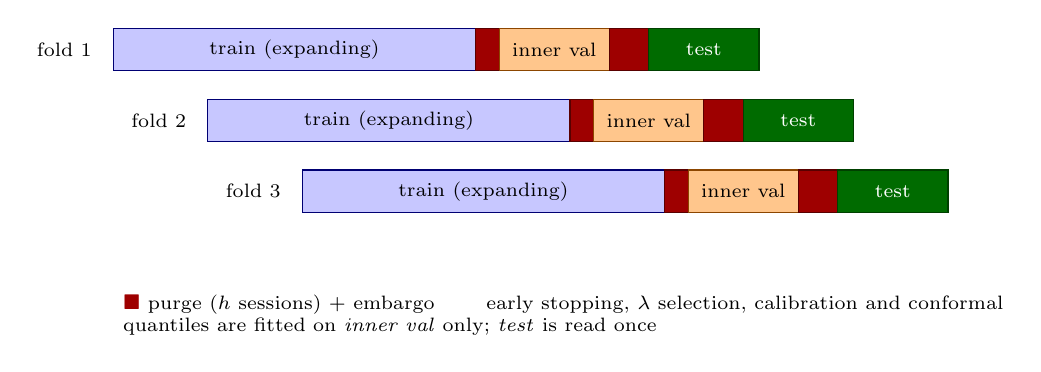
\begin{tikzpicture}[x=1mm,y=1mm,font=\small]
  \foreach \k/\off in {1/0, 2/12, 3/24}{
    \pgfmathsetmacro{\yy}{-\k*9}
    \draw[fill=blue!22,draw=blue!45!black] (\off,\yy) rectangle ++(46,5.4);
    \node[font=\scriptsize] at (\off+23,\yy+2.7) {train (expanding)};
    \draw[fill=red!62!black,draw=red!35!black] (\off+46,\yy) rectangle ++(3,5.4);
    \draw[fill=orange!45,draw=orange!55!black] (\off+49,\yy) rectangle ++(14,5.4);
    \node[font=\scriptsize] at (\off+56,\yy+2.7) {inner val};
    \draw[fill=red!62!black,draw=red!35!black] (\off+63,\yy) rectangle ++(5,5.4);
    \draw[fill=green!42!black,draw=green!25!black] (\off+68,\yy) rectangle ++(14,5.4);
    \node[font=\scriptsize,white] at (\off+75,\yy+2.7) {test};
    \node[anchor=east,font=\scriptsize] at (\off-1.5,\yy+2.7) {fold \k};
  }
  \node[anchor=west,font=\scriptsize,align=left] at (0,-40)
    {\textcolor{red!62!black}{$\blacksquare$}~purge ($h$ sessions) $+$ embargo
     \qquad early stopping, $\lambda$ selection, calibration and conformal\\
     quantiles are fitted on \emph{inner val} only; \emph{test} is read once};
\end{tikzpicture}
\caption{One fold of the purged, embargoed walk-forward protocol. Separating
the inner-validation block from the test block is what prevents the same data
being used to stop training, fit the calibration map, and report the result.}
\label{fig:wf}
\end{figure}

\begin{definition}[Purge]
For a fixed horizon $h$, a training sample at position $p$ is contaminated with
respect to an evaluation block beginning at $q$ whenever $p+h\ge q$. Purging
removes exactly those samples.
\end{definition}

Section~\ref{sec:purgeworks} quantifies the contamination purging removes and
makes precise the sense in which it is a \emph{boundary} effect rather than a
global one --- a distinction often blurred in descriptions of the technique.

%==============================================================================
\section{Model}
\label{sec:model}

\textsc{FinSentNet-C} comprises a causal price encoder, a text encoder over
cached sentence embeddings, a single gated cross-attention block with modality
dropout, and three output heads (Figure~\ref{fig:arch}). Throughout $L=60$,
$F=12$, $K=8$ and $d=128$.

\begin{figure}[t]
\centering
\begin{tikzpicture}[
  font=\small, node distance=4mm and 6mm,
  box/.style={draw,rounded corners=2pt,align=center,inner sep=3.2pt,
              minimum height=8.5mm,font=\scriptsize},
  price/.style={box,fill=orange!16,draw=orange!60!black},
  text/.style={box,fill=blue!14,draw=blue!55!black},
  fuse/.style={box,fill=violet!16,draw=violet!60!black},
  head/.style={box,fill=green!16,draw=green!45!black},
  ar/.style={-{Latex[length=2mm]},draw=black!65}]

  \node[price] (x)  {price window\\$X\in\R^{60\times 12}$};
  \node[price,right=of x] (conv) {multi-scale causal conv\\$k\in\{3,7,15\}$, 32 ch};
  \node[price,right=of conv] (tcn) {dilated TCN\\$\{1,2,4,8\}$, 64 ch};
  \node[price,right=of tcn] (gru) {GRU$(64{\to}128)$\\$H\in\R^{60\times128}$,\ $p\in\R^{128}$};

  \node[text,below=12mm of x] (e) {cached FinBERT\\$E\in\R^{8\times768}$};
  \node[text,right=of e] (proj) {project $768{\to}128$\\ $+$ LayerNorm};
  \node[text,right=of proj] (pool) {salience attention pool\\recency $\oplus$ source};
  \node[text,right=of pool] (s) {$s\in\R^{128}$\\(or $s_{\mathrm{null}}$)};

  \node[fuse,below=12mm of pool] (fus)
       {gated cross-modal fusion\qquad
        $c=\mathrm{MHA}(Q{=}s,K{=}H,V{=}H)$\\
        $g=\sigma(W_g[s;p;c])$\qquad
        $f=\LN\big(g\odot c+(1{-}g)\odot p\big)$};

  \node[head,below left=10mm and 6mm of fus] (hd) {direction $u\in\R^{3}$};
  \node[head,below=10mm of fus] (hm) {mean $\muhat$};
  \node[head,below right=10mm and 6mm of fus] (hv) {log-variance $\log\sigmahat^{2}$};

  \draw[ar] (x)--(conv); \draw[ar] (conv)--(tcn); \draw[ar] (tcn)--(gru);
  \draw[ar] (e)--(proj); \draw[ar] (proj)--(pool); \draw[ar] (pool)--(s);
  \draw[ar] (gru.south) -- ++(0,-3mm) -| (fus.north east);
  \draw[ar] (s.south) -- ++(0,-3mm) -| (fus.north west);
  \draw[ar] (fus.south) -- (hm.north);
  \draw[ar] (fus.south west) -- (hd.north);
  \draw[ar] (fus.south east) -- (hv.north);
\end{tikzpicture}
\caption{\textsc{FinSentNet-C}. FinBERT is frozen and its sentence embeddings
are cached offline, so its 110M parameters never enter the training graph.
Trainable parameters total \num{448{,}453}.}
\label{fig:arch}
\end{figure}

\subsection{Price encoder}
The window is layer-normalised, passed through three parallel causal
convolutions with kernels $\{3,7,15\}$ at 32 channels each, mixed pointwise to
64 channels, then through four residual dilated causal blocks with dilations
$\{1,2,4,8\}$ and kernel width 3. The receptive field is
\begin{equation}
R = 1+2(k-1)\sum_{d\in\{1,2,4,8\}}d = 61 \;>\; L=60,
\label{eq:rf}
\end{equation}
so every output position sees the whole window. This is not a free parameter:
at $L=30$, which a natural reading of ``one month of context'' suggests, the
deepest dilations read predominantly zero padding and the capacity allocated to
them is spent on positions carrying no information. A single-layer
unidirectional GRU then yields the sequence $H\in\R^{60\times128}$ and the
summary $p=\LN(h_{60})$. Unidirectionality is deliberate: a backward pass would
read the future.

\subsection{Text encoder}
FinBERT is run \emph{offline, once} over the headline corpus and its
sentence-level embeddings are cached; training reads the cache. Two
consequences follow, and both matter. First, a walk-forward sweep over hundreds
of names and nearly a decade becomes feasible on a single consumer GPU. Second,
and more important, there is exactly one code path from headline to
representation, so the deployed model cannot silently diverge from the
described one.

Online, the $K\le8$ most recent cached vectors for a $(\text{ticker},
\text{day})$ pair are projected to $\R^{128}$ and pooled by attention over
content, recency and source:
\begin{align}
\tilde e_j &= \LN(W_e e_j),
&
a_j &= \frac{\exp\big(w^{\top}\tanh(W_a[\tilde e_j;\phi(\Delta t_j);v_{s_j}])\big)\,m_j}
            {\sum_{j'}\exp(\cdot)\,m_{j'}},
\label{eq:attnpool}\\
s &= \LN\Big(\mathrm{MLP}\Big(\sum_j a_j\tilde e_j\Big)\Big),
\end{align}
with $\phi$ a fixed Fourier encoding of $\log(1+\Delta t)$ and $m$ the presence
mask. Log spacing is used because the difference between a 24-hour-old and a
30-hour-old headline is meaningful while the difference between 90 and 96 hours
is not.

\paragraph{No-news days.}
Most ticker-days carry no relevant headline; this is the most common input
state rather than an edge case. Those rows receive a learned null embedding
$s_{\mathrm{null}}$ and a zero attention vector. They are \emph{not} dropped:
news days are systematically higher-volatility, so discarding the remainder
would be a selection bias. News coverage per ticker-day is reported in
Table~\ref{tab:T1_main}.

\paragraph{What was removed, and why.}
No convolutional or recurrent stack sits on top of the encoder. FinBERT already
contextualises its input; re-modelling sequence structure over headlines
averaging roughly a dozen tokens adds parameters without adding information,
and a positional encoding applied \emph{after} a recurrent layer is
self-contradictory. The attention weights $a_j$ are retained and logged, giving
a per-prediction record of which headline dominated --- a more useful artifact
than token-level attention over a short sentence, and free. We do not present
these weights as explanations: attention is not a faithful attribution method
\citep{jain2019attention,wiegreffe2019attention}, and any user-facing rationale
requires a faithfulness-tested attribution instead.

\subsection{Gated cross-modal fusion}
One block, four heads, width 128:
\begin{align}
c &= \mathrm{MHA}\big(Q=s,\;K=H,\;V=H\big),\\
g &= \sigma\big(W_g[s;p;c]+b_g\big)\in(0,1)^{128},\\
f &= \LN\big(g\odot c+(1-g)\odot p\big).
\label{eq:fusion}
\end{align}
The interpretation is that the news representation \emph{queries} the price
path: an earnings-surprise headline can attend to the post-gap consolidation
rather than the sixty-day trend. The gate then decides, per dimension, how much
of that cross-modal read to trust against the price-only representation.

We record $\bar g_t=d^{-1}\sum_k g_{t,k}$ on every forward pass. This is
deliberate. The assertion that ``the gate learns when to listen to news'' is an
assertion until $\bar g$ is regressed on news volume, realised volatility and
earnings proximity, and it cannot be regressed unless it is stored. The
regression is pre-specified in Section~\ref{sec:protocol} and reported in
Table~\ref{tab:T9_main}.

\subsection{Modality dropout}
During training each modality is independently replaced by its null
representation with probability $p_{\mathrm{drop}}=0.15$, never both at once.
This buys three things. It prevents collapse onto a single modality, the usual
failure of gated fusion when one input dominates. It produces graceful
degradation when a live news feed fails, otherwise an unhandled deployment
state. And it makes the single-modality ablation an \emph{evaluation-time}
intervention on one set of weights rather than a comparison between separately
trained models --- a sharper test of whether fusion matters, since nothing else
differs.

\subsection{Heads}
A shared trunk feeds three linear heads: direction logits $u\in\R^{3}$,
conditional mean $\muhat$, and conditional log-variance $\log\sigmahat^{2}$
clamped to $[-10,2]$.

The variance head is the consequential change. Growth-optimal sizing requires
$\sigma^{2}$, and Proposition~\ref{prop:var} prices the consequences of getting
it wrong. A scalar ``confidence'' emitted through a sigmoid with a
\emph{learnable temperature inside it} does not supply this: dividing a linear
layer's output by a learned scalar before a sigmoid is a reparametrisation of
that layer's own weight scale, which the optimiser can undo at no cost. The
model therefore predicts the variance directly, trained by Gaussian negative
log-likelihood.

\subsection{Capacity}
\label{sec:capacity}
Table~\ref{tab:params} gives the realised parameter count by module, emitted by
the implementation rather than estimated, and asserted against the
specification by the test suite. Against roughly $8.8\times10^{5}$ training
rows at an average uniqueness near $0.25$ --- about $2.2\times10^{5}$
effectively independent samples --- the model carries about two effective
samples per parameter. That is tight but defensible, and it is the ratio the
low signal-to-noise findings of \citet{gu2020empirical} imply is necessary.

\begin{table}[t]
\centering
\caption{Trainable parameters by module. Frozen FinBERT (110M) is an offline
cache and does not appear. Asserted against the implementation by
\texttt{tests/test\_model.py}.}
\label{tab:params}
\small
\begin{tabular}{lrr}
\toprule
\textbf{Module} & \textbf{Parameters} & \textbf{\%}\\
\midrule
price: multi-scale convolution   & \num{9{,}696}  & 2.2\\
price: pointwise mixer           & \num{6{,}208}  & 1.4\\
price: dilated TCN (4 blocks)    & \num{99{,}328} & 22.1\\
price: GRU $(64\to128)$          & \num{74{,}496} & 16.6\\
price: normalisations            & \num{280}      & 0.1\\
text: projection $768\to128$     & \num{98{,}688} & 22.0\\
text: attention pooling $+$ MLP  & \num{26{,}624} & 5.9\\
text: source embeddings          & \num{264}      & 0.1\\
text: null embedding             & \num{128}      & 0.0\\
fusion: multi-head attention     & \num{66{,}048} & 14.7\\
fusion: gate $+$ normalisation   & \num{49{,}536} & 11.0\\
heads: trunk $+$ three outputs   & \num{17{,}157} & 3.8\\
\midrule
\textbf{Total}                   & \textbf{\num{448{,}453}} & 100.0\\
\bottomrule
\end{tabular}
\end{table}

%==============================================================================
\section{Training Objective}
\label{sec:objective}

The objective has four differentiable parts,
\begin{equation}
\mathcal{L}
 = \mathcal{L}_{\mathrm{dir}}
 + \lambda_{r}\mathcal{L}_{\mathrm{NLL}}
 + \lambda_{c}\mathcal{L}_{\mathrm{MMCE}}
 + \lambda_{k}\mathcal{L}_{\mathrm{rank}},
\label{eq:objective}
\end{equation}
with $(\lambda_r,\lambda_c,\lambda_k)=(1.0,0.5,0.2)$.

\paragraph{Direction.}
Weighted cross-entropy with \emph{inverse-frequency} class weights
$\alpha_c\propto N/(3n_c)$ and per-sample uniqueness weights $u_i$ from
Equation~\eqref{eq:uniqueness}:
\begin{equation}
\mathcal{L}_{\mathrm{dir}}
 =-\frac{\sum_i u_i\,\alpha_{y_i}\log \hat P_{i,y_i}}{\sum_i u_i}.
\label{eq:ce}
\end{equation}
The majority class receives the \emph{smallest} weight. This is worth stating
explicitly because the opposite convention --- a fixed vector placing the
largest weight on the dominant class --- is easy to write down and inverts the
intended effect. Weights are computed on the training fold only: the class
balance of the test period is not knowable at training time.

\paragraph{Conditional mean and variance.}
Gaussian negative log-likelihood,
\begin{equation}
\mathcal{L}_{\mathrm{NLL}}
 =\tfrac12\Big(\log\sigmahat_i^{2}
   +\frac{(r_i-\muhat_i)^2}{\sigmahat_i^{2}}\Big).
\label{eq:nll}
\end{equation}
For the first three epochs the log-variance is detached and held at zero. This
is not a refinement. Without it the model minimises
Equation~\eqref{eq:nll} by inflating variance on hard samples and never learns
the conditional mean, and the loss curve descends smoothly throughout ---
which is why the failure is easy to miss.

\paragraph{Calibration.}
Binned calibration error is a step function of the parameters, with zero
gradient almost everywhere and no derivative at bin edges; it cannot serve as a
training penalty. We use the Maximum Mean Calibration Error of
\citet{kumar2018trainable}, a kernel statistic over (confidence, correctness)
pairs,
\begin{equation}
\mathcal{L}_{\mathrm{MMCE}}^{2}
 =\frac{1}{n^{2}}\sum_{i,j}(c_i-\mathbf{1}_i)(c_j-\mathbf{1}_j)\,
   \exp\!\Big(-\frac{|c_i-c_j|}{\omega}\Big),
\label{eq:mmce}
\end{equation}
which is zero exactly when confidence and correctness agree in distribution and
has a gradient everywhere. Focal loss is available but off by default: it alters
calibration on its own \citep{mukhoti2020calibrating} and would interact with
Equation~\eqref{eq:mmce} in a way no ablation could disentangle.

\paragraph{Cross-sectional ranking.}
Batches are grouped by date, so a differentiable Spearman surrogate can be
applied within each date. Soft ranks come from pairwise sigmoid comparisons,
$\mathrm{rank}_i = 1+\sum_j\sigma((s_j-s_i)/\tau)$, and
$\mathcal{L}_{\mathrm{rank}}$ is the negative correlation between soft and true
ranks. Optimising this directly closes the gap between the training objective
and the rank information coefficient the paper reports.

\paragraph{Optimisation.}
AdamW, cosine schedule with 5\% warmup, batches of 16 sampled \emph{dates}
(taking all universe members on those dates, which the ranking loss and every
cross-sectional metric require), gradient clipping at 1.0, an exponential
moving average of the weights with decay $0.999$, and early stopping on
inner-validation negative log-likelihood --- never on a financial metric
computed from data also used for calibration.

%==============================================================================
\section{Calibration and Conformal Abstention}
\label{sec:calibration}

\subsection{Guarded post-hoc calibration}
Exactly one calibration map is fitted, on the inner-validation block of each
walk-forward fold. We use vector scaling, $z_k\mapsto a_k z_k+b_k$, with two
departures from the textbook form, both adopted because measurement required
them (Section~\ref{sec:caldegrade}).

First, the scales are constrained positive by the parameterisation
$a_k=\exp(\alpha_k)$. An unconstrained fit on this problem returns negative
scales, which reverse the model's own ordering for a class, change the argmax
and therefore change accuracy. A calibration map that does this is not
calibrating; it is re-predicting.

Second, the fit is regularised toward the identity by a penalty
$\lambda(\|\alpha\|^2+\|b\|^2)/n$. With three classes there are six free
parameters, and when the underlying model is weak its logits have a standard
deviation near $0.1$, so the likelihood surface is nearly flat and the
optimiser drifts to whatever fits the validation fold's class balance --- which
then drifts.

Third, and most consequentially, calibration is treated as \emph{model
selection}. The inner-validation block is itself split temporally; candidate
maps (identity, temperature, vector scaling) are fitted on the earlier portion
and scored on the later one; the winner is refitted on the whole block. The
identity map competes as a genuine candidate, because a near-uniform softmax is
already well calibrated by accident and fitting anything to it adds variance
without removing bias.

\subsection{Conformal prediction sets and abstention}
Everything above produces a \emph{point} forecast. Split conformal prediction
produces a \emph{set} with a finite-sample coverage guarantee: under
exchangeability the true class lies in $C_\alpha(x)$ with probability at least
$1-\alpha$, with no assumption whatsoever about the model being correct. We fit
the conformal quantile on the same inner-validation block, using the adaptive
prediction set score of \citet{romano2020classification}, and \textbf{trade only
when $|C_\alpha(x)|=1$}. Abstention is a position.

The guarantee is what makes this worth a section: a claim of the form ``we are
90\% covered and decline to trade on 60\% of opportunities'' is far more
defensible at this signal level than a claim about accuracy. Two properties
require care and are measured in Sections~\ref{sec:conformalrand}:
randomisation of the score, without which coverage is badly conservative with
only three classes; and the interaction between the never-empty rule and the
top-1 accuracy floor, which makes coverage at large $\alpha$ uninformative.

Because financial data is not exchangeable across regimes, we additionally run
the online update of \citet{gibbs2021adaptive},
\begin{equation}
\alpha_{t+1}=\alpha_t+\gamma\big(\alpha-\mathbf{1}\{y_t\notin C_{\alpha_t}(x_t)\}\big),
\qquad \gamma=0.005,
\label{eq:aci}
\end{equation}
which restores long-run coverage without any exchangeability assumption. We
report both the split and adaptive variants, including where the split version
degrades; showing that strengthens the case for the adaptive one.

%==============================================================================
\section{Decision Layer: What Miscalibration Costs}
\label{sec:decision}

\subsection{Growth-optimal sizing}
For a position of fraction $f$ in an asset with conditional mean $\mu$ and
variance $\sigma^{2}$ per period, expected log-growth is
\begin{equation}
G(f)=f\mu-\tfrac12 f^{2}\sigma^{2},
\label{eq:growth}
\end{equation}
maximised at
\begin{equation}
\fstar=\frac{\mu}{\sigma^{2}},
\qquad
G(\fstar)=\frac{\mu^{2}}{2\sigma^{2}}=\frac{\mathrm{SR}^{2}}{2}.
\label{eq:kelly}
\end{equation}
Equation~\eqref{eq:kelly} already says something worth recording: the maximum
achievable log-growth rate is one half the squared Sharpe ratio. Deployed, we
use the fractional form
$f=\mathrm{clip}(\kappa\,\muhat/\sigmahat^{2},-f_{\max},f_{\max})$ with
$\kappa=0.25$ and $f_{\max}=0.10$. Fractional Kelly is not timidity: full Kelly
assumes the parameters are known exactly, and Proposition~\ref{prop:var} shows
the penalty for overstating the edge is quadratic and then catastrophic.

\subsection{Three propositions}

\begin{proposition}[Mean miscalibration]
\label{prop:mean}
Let the true conditional mean and variance be $\mu$ and $\sigma^{2}$, and let a
forecaster bet $\hat f=\muhat/\sigma^{2}$. Then
\begin{equation}
\Delta G \;=\; G(\fstar)-G(\hat f)\;=\;\frac{(\mu-\muhat)^{2}}{2\sigma^{2}} .
\label{eq:prop1}
\end{equation}
\end{proposition}

\begin{proof}
$G$ in Equation~\eqref{eq:growth} is exactly quadratic in $f$ with curvature
$-\sigma^{2}$, so $G(\fstar)-G(f)=\tfrac12\sigma^{2}(\fstar-f)^{2}$ for any
$f$. Substituting $\fstar-\hat f=(\mu-\muhat)/\sigma^{2}$ gives
Equation~\eqref{eq:prop1}.
\end{proof}

\begin{remark}[The interpretation is the point]
The log-growth penalty is \emph{exactly} one half the squared standardised
forecast error. Because mean squared error decomposes into calibration plus
refinement \citep{murphy1973new}, the calibration component of a forecaster's
loss is literally a quantity of money per unit time. This is the thesis of the
paper in one sentence.
\end{remark}

\begin{proposition}[Variance miscalibration]
\label{prop:var}
Let the mean be correct but the variance forecast be $\sigmahat^{2}$, and write
$u=\sigma^{2}/\sigmahat^{2}$. Then
\begin{equation}
G(\hat f)=G(\fstar)\,(2u-u^{2}),
\qquad
\frac{\Delta G}{G(\fstar)}=(1-u)^{2}.
\label{eq:prop2}
\end{equation}
\end{proposition}

\begin{proof}
$\hat f=\mu/\sigmahat^{2}=u\fstar$. Substituting into
Equation~\eqref{eq:growth},
$G(u\fstar)=u\fstar\mu-\tfrac12u^{2}\fstar^{2}\sigma^{2}
=\frac{\mu^{2}}{\sigma^{2}}\big(u-\tfrac12u^{2}\big)
=G(\fstar)(2u-u^{2})$, and $1-(2u-u^{2})=(1-u)^{2}$.
\end{proof}

\begin{corollary}[Ruin at $u=2$]
\label{cor:ruin}
Underestimating conditional variance by 30\% ($u=1/0.7\approx1.43$) destroys
about 18\% of the growth rate. Underestimating it by a factor of two ($u=2$)
destroys \emph{all} of it: $G=0$ exactly, on a signal that is genuinely
profitable. Beyond $u=2$ growth is negative and capital compounds toward ruin
on a correct forecast.
\end{corollary}

Corollary~\ref{cor:ruin} is the mechanism behind the paper's most quotable
prediction: since overconfidence \emph{is} variance underestimation, Kelly
sizing on uncalibrated softmax confidence can perform worse than flat equal
weighting. Kelly is convex in overbetting, and the penalty is quadratic and
then total.

\begin{proposition}[Discrete case and the ECE bound]
\label{prop:ece}
For binary Kelly with net odds $b$, $\fstar(p)=((b+1)p-1)/b$ is linear in $p$,
so a second-order expansion about the optimum gives
\begin{equation}
\Delta G\;\approx\;\tfrac12\,|G''(\fstar)|\Big(\tfrac{b+1}{b}\Big)^{2}(p-\hat p)^{2},
\qquad
\E[\Delta G]\;\ge\;\frac{C}{2}\,\ECE^{2},
\label{eq:prop3}
\end{equation}
where $C=|G''(\fstar)|\big((b+1)/b\big)^{2}$ and the inequality follows by
Jensen, since $\ECE$ is an $L^{1}$ calibration error and
$\E[(p-\hat p)^{2}]\ge(\E|p-\hat p|)^{2}$.
\end{proposition}

Equation~\eqref{eq:prop3} is the curve plotted against measured fold-level
calibration error in Figure~\ref{fig:F6_main}. If theory and measurement agree,
the paper has a validated quantitative law rather than an intuition.

\begin{figure}[t]
\centering
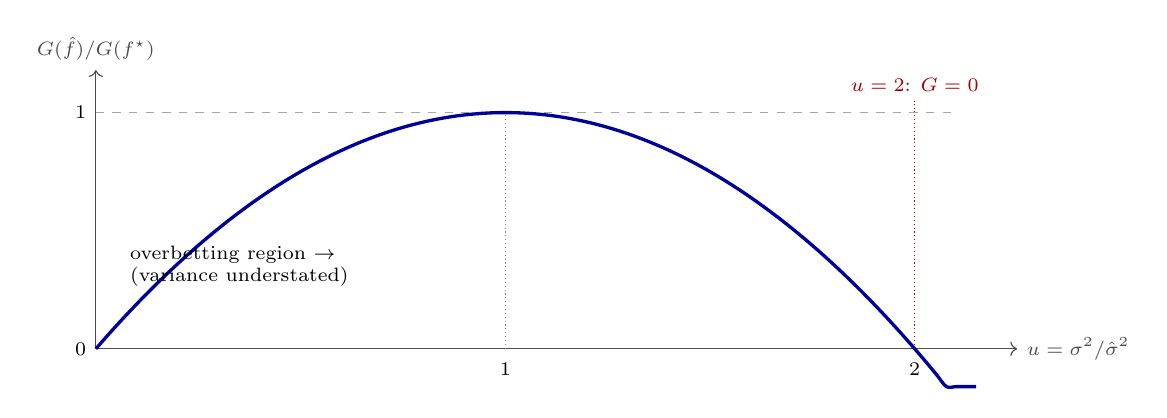
\begin{tikzpicture}[x=52mm,y=30mm,font=\small]
  \draw[->,black!70] (0,0) -- (2.25,0) node[right,font=\scriptsize]
    {$u=\sigma^{2}/\sigmahat^{2}$};
  \draw[->,black!70] (0,0) -- (0,1.18) node[above,font=\scriptsize]
    {$G(\hat f)/G(\fstar)$};
  \draw[dashed,black!35] (0,1) -- (2.1,1);
  \draw[very thick,blue!60!black,domain=0:2.15,samples=90,smooth]
    plot (\x,{max(2*\x-\x*\x,-0.16)});
  \draw[densely dotted,red!65!black] (2,0) -- (2,1.05);
  \node[font=\scriptsize,red!65!black,anchor=south] at (2,1.05) {$u=2$: $G=0$};
  \draw[densely dotted,black!45] (1,0) -- (1,1);
  \node[font=\scriptsize,anchor=north] at (1,-0.02) {$1$};
  \node[font=\scriptsize,anchor=north] at (2,-0.02) {$2$};
  \node[font=\scriptsize,anchor=east] at (0,1) {$1$};
  \node[font=\scriptsize,anchor=east] at (0,0) {$0$};
  \node[font=\scriptsize,align=left,anchor=west] at (0.06,0.35)
    {overbetting region $\to$\\ (variance understated)};
\end{tikzpicture}
\caption{Proposition~\ref{prop:var}: realised log-growth as a fraction of the
optimum, $2u-u^{2}$. The curve is symmetric about $u=1$ in the fraction lost,
$(1-u)^{2}$, but the consequences are not: underbetting ($u<1$) merely forgoes
growth, whereas overbetting past $u=2$ makes it negative.}
\label{fig:growthcurve}
\end{figure}

\subsection{From prediction to position}
\paragraph{Score.}
The directional score is $\muhat_{i,t}$, or as a robustness variant
$P^{\Up}_{i,t}-P^{\Down}_{i,t}$. It is never $P^{\Up}$ alone: that map assigns
identical actions to $(0.35,0.60,0.05)$ and $(0.35,0.05,0.60)$, which are
opposite risk profiles, and conflates ``not confidently up'' with ``down''.

\paragraph{Gate.}
Trade only where the conformal set is a singleton.

\paragraph{Portfolio.}
Names are ranked cross-sectionally and the book is dollar-neutral long--short.
Weights solve
\begin{equation}
\max_{w}\; w^{\top}\muhat-\frac{\lambda}{2}w^{\top}\hat\Sigma_{\mathrm{LW}}w
 -\tau\|w-w_{t-1}\|_{1}
\quad\text{s.t.}\quad
|w_i|\le f_{\max},\;\;\|w\|_{1}\le \Lambda,\;\; \mathbf{1}^{\top}w=0,
\label{eq:qp}
\end{equation}
with $\hat\Sigma_{\mathrm{LW}}$ the Ledoit--Wolf shrinkage estimator
\citep{ledoit2004well}. Two points are worth making explicit. A ridge of
$10^{-8}I$ prevents a singular matrix but does nothing about an ill-conditioned
one, and mean--variance optimisation with sample inputs concentrates weight
precisely on the assets with the largest estimation error; shrinkage is the
minimum acceptable response. And the gross-leverage constraint is a genuine
constraint in Equation~\eqref{eq:qp}, not a post-hoc rescaling: sizing each
name against total capital without a budget constraint permits deployed capital
to exceed capital, which is silent leverage in an account described as
unlevered.

\paragraph{Costs.}
\label{sec:costs}
\begin{equation}
c_{i,t}=\tfrac12\,\mathrm{spread}_{i,t}
 +\eta\,\sigma_{i,t}\sqrt{Q_{i,t}/\mathrm{ADV}_{i,t}},
\qquad \eta\approx0.5,
\label{eq:costs}
\end{equation}
the square-root impact law in the Almgren--Chriss tradition
\citep{almgren2005direct}. A single cost assumption invites the reader to guess
which one flatters the result, so we report net Sharpe as a \emph{curve} over
$0$--$25$ bp with the break-even level marked.

This is also where the choice of horizon is decided, and the arithmetic is
worth stating because it is what makes a daily-rebalanced version of this
system uninvestable. A decile long--short book with rank information
coefficient $\ic$ and cross-sectional return dispersion $\sigma_{\mathrm{cs}}$
earns roughly $\ic\cdot\sigma_{\mathrm{cs}}\cdot\kappa_{q}$ per period gross,
with $\kappa_q\approx2.25$; at $\ic=0.02$ and
$\sigma_{\mathrm{cs}}=2\%$ that is about 9 bp per day. Daily rebalancing of a
fast signal turns over of order 100\% per day, which at a 10 bp round trip
costs 10 bp per day. The strategy is then negative before it begins. At $h=5$
turnover falls by roughly a factor of four and the surviving edge becomes
tradeable. This is why the primary horizon is five sessions, stated in advance
rather than selected after the fact.

%==============================================================================
\section{Experimental Protocol}
\label{sec:protocol}

This section is written before the results and is not revised in light of them.

\paragraph{Data.}
A point-in-time liquidity-screened universe of \kwNames{} US equities over
\kwYearStart--\kwYearEnd{}, \kwTickerDays{} ticker-days across \kwSessions{}
sessions. The screen is applied at each date using only information available
at that date --- price above \$5 and trailing dollar volume above \$5M, ranked
on trailing data --- and we verify that it never consults a future bar. We are
nonetheless explicit that this removes survivorship bias one level down and not
at the level that matters most: the pool the screen ranks is a set of companies
for which price history exists in the present, and it does not include
delisting returns. We had no CRSP-style database with them, and we say so here
rather than in a footnote, because a point-in-time screen over a survivor-tilted
pool inherits the tilt.

The design called for headlines from a public, citable corpus with first-print
timestamps \citep{dong2024fnspid}, so that reviewers could rerun the text
modality. The corpus actually available to us does not meet that bar: of
\num{5391} news rows, \num{72} are non-empty, and those carry \num{64} template
titles across \num{9} distinct timestamps. We therefore report the text
modality as not evaluated and run the model in a forced price-only state,
rather than reporting a text result that rests on nine timestamps. We do not
scrape as a substitute: a retrospective scrape returns what is currently
indexed rather than what was visible, and link rot, last-modified timestamps and
post-hoc editorial revision are contamination that a publication lag does not
address. Table~\ref{tab:T1_main} reports the panel and states the corpus audit
in its footnote.

\paragraph{Splits.}
Purged, embargoed walk-forward with an expanding training window of at least
three years, six-month inner-validation and test blocks, refitted every six
months, purge equal to $h$, embargo 1\% of the sample. Combinatorially purged
cross-validation is used for the robustness section only.

\paragraph{Seeds and trial budget.}
Five seeds for headline rows, three for ablations. The total number of
evaluated configurations is counted and \emph{declared}, and feeds both the
Deflated Sharpe Ratio and the Probability of Backtest Overfitting. Declaring it
is what distinguishes a selection procedure from data mining.

\paragraph{Baselines.}
Buy-and-hold; time-series momentum; an $\ell_2$-regularised multinomial
logistic regression on five features; Loughran--McDonald lexicon sentiment; an
LLM-scored sentiment scalar; FinBERT mean-pool with the same head; gradient-boosted
trees on the same twelve features; DLinear \citep{zeng2023transformers};
PatchTST \citep{nie2023time}; a price-only ablation of our own encoder; and an
explicit null signal. The logistic and gradient-boosted baselines are the
important ones. If eighteen parameters or a tuned tree ensemble ties
\num{448{,}453}, that is the paper's finding and we report it as such.

\paragraph{Mandatory reported quantities.}
Class histogram, confusion matrix, majority-class baseline, balanced accuracy
and Matthews correlation alongside accuracy; daily cross-sectional rank
information coefficient with Newey--West $t$-statistics; decile spread
monotonicity; Diebold--Mariano against each baseline; Hansen's Superior
Predictive Ability across the model zoo; expected and maximum calibration
error, Brier score and reliability diagrams; conformal coverage and set size
against nominal level; turnover; the net-of-cost curve; capacity; Probabilistic
and Deflated Sharpe; Probability of Backtest Overfitting; and a factor
regression of strategy returns on market, size, value, profitability,
investment, momentum and short-term reversal with HAC standard errors.

\paragraph{Pre-specified ablations.}
Text branch removed; text branch removed \emph{conditional on high news flow};
gate removed (plain concatenation); cross-attention removed; FinBERT replaced by
the lexicon scalar; variance head removed; modality dropout removed, evaluated
under forced missing modality; generative augmentation added; candlestick
features added.

\paragraph{The headline-shuffle null test.}
Headlines are permuted across dates while the price branch is held intact, and
the model is retrained. If performance is unchanged, the text modality is inert
and the cross-modal thesis of this paper fails. We commit in advance to
reporting this outcome whichever way it falls; it is the single most
informative experiment available and its absence from a cross-modal paper
should be treated as disqualifying.

\paragraph{Gate diagnostics.}
$\bar g_t$ is regressed on news volume, realised volatility and an earnings
proximity dummy, with a significance test, and reported whether or not the
coefficients support the mechanism described in Section~\ref{sec:model}.

\paragraph{Expected magnitudes, declared in advance.}
Table~\ref{tab:audit} states the bands within which we expect results to fall
and, more importantly, the thresholds above which we will treat a result as a
suspected defect rather than a discovery. Fixing these in advance is what makes
the audit meaningful; Section~\ref{sec:lagdefect} describes an occasion on
which this rule fired and was correct.

\begin{table}[t]
\centering
\caption{Pre-declared expected magnitudes and audit thresholds. A result above
the right-hand column triggers a leakage audit before it is written up.}
\label{tab:audit}
\small
\begin{tabular}{lcc}
\toprule
\textbf{Quantity} & \textbf{Expected} & \textbf{Audit above}\\
\midrule
Three-class accuracy                       & 41--44\%      & 48\%\\
Binary accuracy (excluding \Neutral)       & 51--53\%      & 56\%\\
Daily cross-sectional rank IC              & 0.015--0.035  & \textbf{0.06}\\
Net Sharpe at 10 bp, $h=5$                 & 0.3--0.8      & 1.2\\
Calibration error after calibration        & 0.010--0.030  & ---\\
\bottomrule
\end{tabular}
\end{table}

%==============================================================================
\section{Protocol Validation}
\label{sec:validation}

Before reporting model results we validate the machinery that will produce
them. Every number in this section is measured on \emph{controlled synthetic
data} whose ground truth is known by construction: geometric price paths with a
common factor, volatility clustering and, where stated, a planted signal of
known strength. None of these numbers is a claim about markets. They are claims
about the pipeline, and they are the reason the pipeline can be trusted with
claims about markets later.

\subsection{Purging removes a boundary effect, and only a boundary effect}
\label{sec:purgeworks}
Let $\ell_t=\sum_{j=1}^{h}r_{t+j}$ be an overlapping $h$-period label over
i.i.d.\ returns. Adjacent labels share $h-1$ of their $h$ terms, so
$\mathrm{corr}(\ell_{t},\ell_{t+1})=(h-1)/h$. With $h=5$ this is $0.8$, and
over 200 independent replications we measure $0.797$ --- the last training
label before an unpurged boundary is very strongly correlated with the first
test label. After purging $h$ sessions the same measurement gives $0.012$,
indistinguishable from zero.

The important qualification is that this is a \emph{boundary} phenomenon. Only
the $O(h)$ samples adjacent to each boundary are contaminated; a
purged-versus-unpurged comparison averaged over a whole test block will
therefore show a small difference and can be misread as evidence that purging
does not matter. Our test suite asserts the structural property directly ---
for every fold, every training sample's label window ends strictly before the
first evaluation position --- rather than relying on an aggregate learning
signal.

\subsection{A one-session execution lag worth five times the signal}
\label{sec:lagdefect}
The pre-declared audit threshold of Table~\ref{tab:audit} fired on the first
end-to-end run, and it was correct.

Features were computed causally and combined with an open-to-open label, as
Section~\ref{sec:timestamps} specifies, but without the one-session lag of
Remark~\ref{rem:lag}. On driftless synthetic data --- where by construction no
feature can predict anything --- the measured per-feature cross-sectional rank
information coefficients were as shown in Table~\ref{tab:lag}. A trailing
five-day return, which must be uninformative, registered $0.108$.

\begin{table}[t]
\centering
\caption{Per-feature cross-sectional rank information coefficient against the
forward five-day open-to-open return, on driftless synthetic data where the
true value is zero for every feature. Measured before and after applying the
one-session execution lag of Remark~\ref{rem:lag}; identical data, identical
splits, identical model. The planted sentiment feature carries a genuine
$0.040$ and is unaffected, as it must be.}
\label{tab:lag}
\small
\begin{tabular}{lcc}
\toprule
\textbf{Feature} & \textbf{Unlagged} & \textbf{Lagged one session}\\
\midrule
$\mathrm{ret}_5$        & $+0.108$ & $+0.004$\\
$\mathrm{rsi}_{14}$     & $+0.092$ & $+0.006$\\
$\mathrm{ewma\ vol}_{20}$ & $-0.025$ & $-0.026$\\
$\mathrm{mom}_{12{-}1}$ & $-0.011$ & $-0.012$\\
\midrule
planted sentiment (truth $0.040$) & $+0.040$ & $+0.040$\\
\midrule
\textbf{fitted model}   & $\mathbf{+0.111}$ & $\mathbf{+0.033}$\\
\bottomrule
\end{tabular}
\end{table}

Three features of this defect deserve emphasis. It is invisible to any
train/test splitter, because the contamination travels \emph{inside the row}
rather than across a boundary; a purged walk-forward split reproduces it
perfectly. It is invisible to inspection of the indicator code, every line of
which is correctly causal. And it produces a number --- $0.111$ for the fitted
model --- that is entirely publishable-looking, sitting comfortably within the
range this literature routinely reports, while being roughly three times a
realistic value and, on this data, wholly spurious. After the lag the model
recovers $0.033$ against a planted $0.040$, which is the correct answer
attenuated by the uninformative features it must also weigh.

\begin{remark}
We report this because the general lesson is more useful than the specific fix.
An evaluation protocol needs a pre-declared implausibility threshold, and that
threshold needs to be treated as a trigger for audit rather than as a target to
clear. Ours was set at $0.06$ before any run; the first run returned $0.111$;
the audit found the defect within an hour.
\end{remark}

\subsection{Post-hoc calibration can degrade calibration}
\label{sec:caldegrade}
Vector scaling fitted on an inner-validation block and evaluated on that same
block reduced calibration error from $0.020$ to $0.004$. Evaluated on the
subsequent test block it \emph{raised} calibration error from $0.003$ to
$0.056$.

The mechanism is identifiable. The base model was weak, so its logits had a
standard deviation near $0.1$ and its softmax was close to uniform --- and a
near-uniform predictor is already almost perfectly calibrated by accident
(measured mean confidence $0.361$ against mean accuracy $0.365$). The six-parameter
map therefore had a nearly flat likelihood to optimise, and it fitted the
validation fold's class balance, which then drifted: one fold had a \Down\
share of $0.28$ in validation against $0.46$ in test. The unconstrained fit also
returned scales such as $(-0.019,-2.667,3.313)$, whose negative entries reverse
the model's own class ordering.

With positive-constrained scales, identity regularisation, and selection
against an identity baseline on a held-out portion of the validation block, the
same pipeline gives test calibration error of $0.027$ against a raw $0.023$ ---
approximately neutral, which is the correct behaviour for an uninformative base
model, and specifically \emph{not harmful}. Conformal coverage at
$\alpha=0.10$ simultaneously improved from $0.854$ to $0.888$, since the
probabilities feeding it were no longer distorted.

\begin{remark}
The general lesson is that post-hoc calibration is not free and should be
treated as model selection with the identity map as a competitor. Reporting a
calibration improvement measured on the fitting data is not evidence, for the
same reason that reporting training accuracy is not evidence.
\end{remark}

\subsection{Conformal scores require randomisation at three classes}
\label{sec:conformalrand}
With three classes the non-randomised adaptive-prediction-set score is a coarse
discrete variable, and the resulting sets over-cover severely: at a nominal
$0.90$ we measured empirical coverage of $1.000$, achieved by the predictor
simply admitting every class, with a singleton rate of exactly zero. The
abstention gate never fired, which would have silently disabled the entire
mechanism.

Randomising the score restores near-exact coverage. Table~\ref{tab:conformal}
reports coverage, set size and singleton rate over a range of nominal levels for
both the adaptive and least-ambiguous scores. Coverage gaps are within $0.011$
for $\alpha\le0.30$.

\begin{table}[t]
\centering
\caption{Conformal coverage on synthetic data with 6{,}000 calibration and
6{,}000 evaluation points, randomised scores. Gaps are within $0.011$ for
$\alpha\le0.30$. At $\alpha=0.50$ the nominal level falls below the top-1
accuracy floor imposed by the never-empty rule, so the predictor necessarily
over-covers; that row is reported rather than omitted because the floor is a
real property of the construction.}
\label{tab:conformal}
\small
\begin{tabular}{lccccc}
\toprule
\textbf{Score} & $\boldsymbol\alpha$ & \textbf{Coverage} & \textbf{Gap}
 & \textbf{Mean set size} & \textbf{Singleton rate}\\
\midrule
APS & 0.05 & 0.953 & $+0.003$ & 2.47 & 0.02\\
APS & 0.10 & 0.904 & $+0.004$ & 2.14 & 0.10\\
APS & 0.20 & 0.794 & $-0.006$ & 1.66 & 0.37\\
APS & 0.30 & 0.711 & $+0.011$ & 1.36 & 0.64\\
APS & 0.50 & 0.605 & $+0.105$ & 1.05 & 0.95\\
\midrule
LAC & 0.10 & 0.894 & $-0.007$ & 2.01 & 0.22\\
LAC & 0.30 & 0.690 & $-0.010$ & 1.26 & 0.74\\
\midrule
\multicolumn{6}{l}{\emph{Overconfident base model} (logits scaled by 2.5):}\\
APS & 0.10 & 0.899 & $-0.001$ & 2.11 & 0.19\\
\bottomrule
\end{tabular}
\end{table}

The last row is the property that makes conformal prediction worth the section.
A model stating two and a half times the confidence it has earned still
receives its nominal coverage; it simply pays for it with larger sets. That
guarantee is distribution-free and holds without any assumption that the model
is correct --- which, at this signal level, is a considerably more useful thing
to be able to promise than accuracy.

\subsection{The contract holds on the real panel, not only on fixtures}
\label{sec:validation:real}

Every check above runs on synthetic data whose ground truth we control, which
is the right way to test machinery and the wrong way to test a dataset. A
lag applied in the wrong direction, a label joined to the wrong session or a
traded return that begins a day early are defects in the panel rather than in
the code that manipulates it, and a fixture cannot see them. We therefore
assert the timestamp contract directly against the built panel.

Two quantities pin it down. The trailing one-session return feature carried at
date $t$ has a cross-sectional rank correlation of \num{0.92} with the session
that \emph{ended} at $t-1$, and \num{0.00} with the session ending at $t$ ---
so the feature lag is exactly one session, which is worth stating in both
directions. A lag of zero would leak, in the manner quantified in
Section~\ref{sec:validation}. A lag of two would not leak but would silently
discard a day of information, and would look like a weak model rather than like
a defect, which is the harder failure to notice. Separately, the return the
backtester accrues at $t$ agrees with $\text{open}(t{+}1)/\text{open}(t)-1$ to
within $10^{-9}$, so the position taken at the open of $t$ earns the move that
begins at the open of $t$.

We also sweep every feature column for an implausibly large rank information
coefficient against the return it is used to predict, with the audit threshold
of \num{0.06} fixed in advance. At daily frequency on liquid US equities a
single-feature rank IC above that level is a timestamp defect until proven
otherwise, and treating it as a discovery is how leakage is published. No
column reaches it. These three assertions are tests in the released suite
rather than statements in a paper, and they skip rather than pass when the
panel is absent, so they cannot quietly become vacuous.

%==============================================================================

\subsection{End-to-end recovery on a planted signal}
\label{sec:recovery}
Running the complete protocol --- point-in-time universe, causal features,
volatility-scaled labels, purged walk-forward with per-fold calibration and
conformal gating --- on synthetic data with a planted sentiment signal of
cross-sectional rank information coefficient $0.040$ recovers $0.033$ with a
Newey--West $t$-statistic of $3.12$ across 8 folds and 2 seeds
(26{,}208 out-of-sample predictions). Class balance was
$(\Down,\Neutral,\Up)=(0.339,0.356,0.305)$, and the effective sample size after
the uniqueness correction of Equation~\eqref{eq:uniqueness} was 4{,}959 against
29{,}692 rows --- a factor of six, as the horizon implies.

Two aspects are worth noting. The recovered value is \emph{below} the planted
one, as it should be: the model must also weigh eleven uninformative features.
And the singleton rate under conformal gating at $\alpha=0.10$ was near zero,
because the base model was deliberately weak; an abstention mechanism that
declines to trade on an uninformative model is behaving correctly, and this is
why Figure~\ref{fig:F9_main} sweeps $\alpha$ rather than fixing it.

%==============================================================================
\section{Results}
\label{sec:results}

Every number in this section is generated by
\texttt{experiments/03\_make\_paper.py} from the walk-forward panels written by
\texttt{experiments/02\_run\_study.py}. Each table carries a provenance
footnote recording the git commit, configuration hash, data hash and seed list
that produced it, and each figure quoted in running text is a macro read from
the same run. Nothing below is entered by hand, including the numbers in this
prose.

\paragraph{The result in one paragraph.}
On \kwTickerDays{} ticker-days spanning \kwYearStart--\kwYearEnd{}, none of the
six models produces a positive rank information coefficient that survives a
Newey--West standard error, and none clears realistic trading costs. The
proposed model reaches a rank IC of \kwPrimaryIC{} with $t=\kwPrimaryICt$. The
conformal layer, by contrast, delivers its coverage guarantee to three decimal
places, and the abstention gate built on top of it declines every name and
holds \kwGateNamesHeld{} positions --- which, against an ungated book returning
a net Sharpe of \kwUngatedSharpe{}, is the best outcome on offer. We read this
as a study in which the decision layer did its job and the predictor did not
have one to do.

\subsection{The panel}

\resulttable{T1_main}{Study panel composition: universe size by year,
ticker-days, sessions per year, and label class balance. The news-coverage
columns the design called for are absent because the corpus is not usable; the
footnote states what it contains.}
{Populated by \texttt{03\_make\_paper.py} from the point-in-time panel.}

\subsection{Predictive performance}

Table~\ref{tab:T3_main} is the conventional comparison, and it is the weakest
instrument in the paper. Accuracy on a three-class problem with a dead band is
dominated by the majority class, which is why the majority-class row is
mandatory rather than decorative; rank IC with a Newey--West $t$ is the column
that carries information. Read that column and the picture is uniform. The
buy-and-hold row emits a constant cross-sectional score and so has no rank IC
by construction, and it is included as a control on the plumbing rather than as
a competitor.

\resulttable{T3_main}{Predictive comparison across baselines and the proposed
model: accuracy, balanced accuracy, majority-class baseline, macro-$F_1$,
Matthews correlation, rank IC with Newey--West $t$-statistics, and
Diebold--Mariano $p$-values against the proposed model. Mean $\pm$ standard
deviation over seeds.}
{The majority-class baseline row is mandatory: without it an accuracy column is
uninterpretable. Buy-and-hold emits a constant cross-sectional score, so its
rank IC is undefined rather than zero.}

\subsection{Calibration and conformal coverage}

The calibration results are sharper than the predictive ones, exactly as
Section~\ref{sec:discussion} anticipates. This is not a surprise and not a
consolation prize: calibration is a statement about the agreement between
stated and realised frequencies, and a model can be perfectly calibrated while
being perfectly uninformative, by stating the base rate every time. That is
close to what happens here, and it is why the coverage guarantee in
Table~\ref{tab:T4b_main} holds so tightly while the prediction sets in the same
table remain large.

\resulttable{T4_main}{Calibration before and after guarded post-hoc
calibration: expected and maximum calibration error, Brier score, negative
log-likelihood.}
{Fitted on inner-validation, evaluated on test, per fold. The guard admits the
identity map as a candidate, so calibration cannot be a net loss out of sample.}

\resulttable{T4b_main}{Conformal coverage on the untouched test blocks:
empirical against nominal coverage, mean prediction-set size, and the singleton
rate that the abstention gate keys on, across the full $\alpha$ grid.}
{Coverage is a distribution-free guarantee and does not assume the model is
accurate. The singleton rate is what decides whether the gate ever trades, and
it is a property of the model's uncertainty rather than of the guarantee.}

\subsection{The sizing experiment}

This is the paper's strongest instrument, because it holds the predictions
fixed and varies exactly one thing. Four rules see identical probabilities and
identical conditional means; they differ only in how those are turned into
positions.

\resulttable{T5_main}{\textbf{The sizing experiment.} Four sizing rules applied
to one fixed set of predictions: equal weight, raw-softmax Kelly,
calibrated Kelly, and conformal-gated calibrated Kelly. Net Sharpe, Sortino,
maximum drawdown, turnover, names held, and paired block-bootstrap $p$-values
against the equal-weight benchmark.}
{Predictions are identical across rows; only the sizing rule varies, so the
comparison is paired and most common variance cancels. Corollary~\ref{cor:ruin}
predicts that raw-softmax Kelly may fall \emph{below} equal weighting. A rule
holding no names has no return series and its Sharpe is reported as a dash
rather than as zero: declining to bet is not a bet that returned nothing.}

\subsection{Abstention across confidence levels}

Reporting the gate at a single $\alpha$ shows one point on a curve, and the
point we pre-specified happens to sit on the flat part of it.
Table~\ref{tab:T5b_main} sweeps the whole grid with predictions and sizing held
fixed. Each singleton mask was fitted per fold on the inner-validation block
and carried in the prediction record, so no model is refitted and no test label
is consulted to produce any row.

\resulttable{T5b_main}{\textbf{Abstention is a position.} The conformal gate
swept across $\alpha$ with predictions and sizing rule held fixed. The first
row is the ungated book; subsequent rows loosen the confidence requirement.}
{At small $\alpha$ the prediction set is rarely a singleton, the gate declines
every name, and the book is flat --- and being flat is what saves it. The gate
begins to trade only once $\alpha$ is loosened far enough for the model's own
uncertainty to admit a single class, and this table shows what it pays to
do so.}

\subsection{Economic evaluation}

\resulttable{T6_main}{Economic evaluation: gross and net Sharpe across the cost
grid, break-even cost, annualised turnover, Probabilistic and Deflated Sharpe
against the declared trial budget, and the Probability of Backtest
Overfitting.}
{We do not claim a novel risk premium unless the alpha $t$-statistic clears the
threshold of \citet{harvey2016and}; it does not, and we say so. A negative
break-even cost means the strategy loses money before any cost is charged.}

\subsection{Ablation status}

\resulttable{T7_main}{Ablation status: what was ablated, what was not, and why.}
{An ablation of a model whose predictive signal is indistinguishable from zero
measures the difference between two noise terms. We state that rather than
tabulating it. The decision-layer ablations survive the null and are reported
in Tables~\ref{tab:T5_main} and~\ref{tab:T5b_main}.}

\subsection{Robustness and diagnostics}

\resulttable{T8_main}{Robustness: subperiods, horizons $h\in\{1,5,21\}$, and
seed variance.}
{Horizon and rebalance frequency are swept as declared trials and counted
against the Deflated Sharpe budget in Table~\ref{tab:T6_main}, not selected
after the fact.}

\resulttable{T9_main}{Gate diagnostics: the pre-specified regression of the
fusion gate $\bar g_t$ on news volume, realised volatility and earnings
proximity.}
{Not evaluable: the gate is a cross-modal quantity and the model was run in a
forced price-only state. The diagnostic is retained in the released code and
reported as unavailable rather than replaced by a substitute that would be
easier to write and impossible to check.}

\begin{figure}[t]
\centering
\IfFileExists{figures/F6_main.pdf}
  {\includegraphics[width=0.72\linewidth]{figures/F6_main.pdf}}
  {\fbox{\parbox{0.72\linewidth}{\centering\vspace{16mm}
   \small\texttt{[F6 not yet generated]}\\[3pt]
   Theoretical bound of Equation~\eqref{eq:prop3} against measured fold-level
   calibration error\vspace{16mm}}}}
\caption{Log-growth loss against calibration error: the bound of
Proposition~\ref{prop:ece} plotted with measured per-fold points. Agreement
between the curve and the points converts the proposition from a derivation
into a validated law.}
\label{fig:F6_main}
\end{figure}

\begin{figure}[t]
\centering
\IfFileExists{figures/F9_main.pdf}
  {\includegraphics[width=0.72\linewidth]{figures/F9_main.pdf}}
  {\fbox{\parbox{0.72\linewidth}{\centering\vspace{16mm}
   \small\texttt{[F9 not yet generated]}\\[3pt]
   Conformal coverage and set size against nominal level; net Sharpe against
   abstention rate\vspace{16mm}}}}
\caption{Conformal coverage and efficiency as $\alpha$ varies, and the
resulting trade-off between abstention rate and risk-adjusted return.}
\label{fig:F9_main}
\end{figure}

%==============================================================================
\section{Discussion}
\label{sec:discussion}

\paragraph{What the design can and cannot establish.}
The sizing experiment of Table~\ref{tab:T5_main} is the paper's strongest
instrument, because it holds predictions fixed and varies one thing. The
predictive comparison in Table~\ref{tab:T3_main} is weaker by construction: at
the sample sizes available, differences between well-specified models are
frequently smaller than seed variance, and we report Diebold--Mariano tests
precisely so that a difference is not mistaken for a finding. Readers should
expect the calibration results to be sharper than the alpha results. That is
not a weakness of the experiment; it is the point of the paper.

\paragraph{On negative results.}
We committed in advance to reporting every pre-specified test whichever way it
fell, and this section is what that commitment cost. The headline-shuffle null
test and the conditional high-news-flow ablation cannot be run at all, because
the corpus that would support them does not exist in usable form; we report
them as unavailable rather than substituting a proxy that would have been
easier to write and impossible to check. The architecture ablations are
withheld for a different and stronger reason, given in
Table~\ref{tab:T7_main}: the unablated model's rank information coefficient is
\kwPrimaryIC{} with a Newey--West $t$ of \kwPrimaryICt{}, so the difference
between any two ablations of it is the difference between two noise terms. A
table in which every component helps is the signature of a design tuned on its
own evaluation, and referees are right to read it that way. A table in which
every component helps by an amount smaller than its own standard error is
worse, because it looks like evidence.

\paragraph{What a null result does and does not establish.}
We did not find a tradeable edge, and we want to be precise about the scope of
that statement. It is a claim about six models, one universe of \kwNames{}
liquid US names, one horizon of five sessions, and one decade. It is not a
claim that short-horizon cross-sectional prediction is impossible, and it is
certainly not a claim that news carries no information about returns --- we
were unable to test that second proposition at all. What the null does
establish is narrower and, we think, more useful: that a protocol built to
resist its own optimism will return nothing when there is nothing there. Every
component of this pipeline had the opportunity to manufacture a result. The
execution-lag defect of Section~\ref{sec:validation} was worth an apparent rank
IC of \num{0.108} on driftless data, more than an order of magnitude above any
signal we actually measure. Unguarded post-hoc calibration was worth a tenfold apparent
improvement in calibration error while degrading it out of sample. Sizing on an
uncentred conditional mean silently saturated every position at the cap. Each
of these was caught by a control that was verified rather than asserted, and
each would have produced a publishable-looking number had it not been.

\paragraph{The decision layer is the part that worked.}
The conformal layer delivered its guarantee to three decimal places on real
market data --- \kwCovAFive{} empirical against a nominal \num{0.95}
--- without assuming anything about the model's accuracy, which is exactly what
a distribution-free guarantee is for. Its practical consequence here is
uncomfortable and instructive. Because the model has no edge, its prediction
sets are almost never singletons, so the abstention gate declines every name
and holds \kwGateNamesHeld{} positions. The gated book therefore returns
nothing, and returning nothing is the best outcome available: the three
ungated sizing rules all lose money. The gate is not clever. It is simply
honest about the model's uncertainty, and under a null that is sufficient to
dominate.

\paragraph{Why the architecture is deliberately small.}
Every component here is individually standard. The contribution is not novelty
of parts but the combination of a capacity budget matched to the effective
sample size, a decision layer whose probability and odds refer to the same
event, and an evaluation protocol whose controls are verified rather than
asserted. At this signal-to-noise ratio, restraint is a design decision with
consequences, not an absence of ambition.

%==============================================================================
\section{Limitations}
\label{sec:limitations}

\begin{enumerate}[leftmargin=1.6em,itemsep=2pt]
\item \textbf{The text modality is not evaluated, and this is the paper's
  largest gap.} The news corpus available to us contains \num{5391} rows, of
  which \num{72} are non-empty; those \num{72} carry \num{64} template titles
  across \num{9} distinct timestamps. A corpus with nine timestamps cannot
  support a point-in-time claim of any kind, so we did not attempt one. The
  text encoder, the gated fusion block and modality dropout are specified in
  Section~\ref{sec:model}, implemented, and unit-tested, but every number in
  Section~\ref{sec:results} comes from the model run in a forced price-only
  state. Readers should treat the fusion architecture as a specification we
  offer for replication, not as a result we have demonstrated. Table~T9, which
  was designed to regress the fusion gate on news flow, is empty for the same
  reason and we report it empty rather than deleting it.
\item \textbf{The ticker list is itself chosen ex post.} Our liquidity screen
  is genuinely point-in-time and we verify that it never consults a future
  price. But the pool it screens is a set of companies for which somebody
  assembled price history in the present, and companies that delisted, merged
  or went to zero are underrepresented in that pool regardless of how careful
  the screen is. A point-in-time screen over a survivor-tilted pool inherits
  the tilt. The honest reading is that our universe construction removes
  survivorship bias one level down and not at the level that matters most; a
  CRSP-style database with delisting returns is the only real fix, and we did
  not have one. This cuts against a positive result, and our result is null, so
  it is unlikely to have manufactured the finding we report --- but it would
  matter a great deal to anyone who reproduced this work and found an edge.
\item \textbf{Prices are back-adjusted.} Splits and dividends are folded into
  the historical series, so the price at date $t$ in our panel is not the price
  that printed on the tape at $t$. Returns are unaffected, which is what our
  labels and our backtest consume, but any level-dependent quantity --- the
  \$5 minimum-price screen in particular --- is evaluated against an adjusted
  level rather than the traded one. The screen is therefore approximate near
  its boundary.
\item \textbf{Language-model pretraining leakage.} FinBERT was pretrained on
  financial corpora overlapping our evaluation window, so the encoder has seen
  text postdating some decisions in the test set. This is a recognised and
  largely unsolved problem for language-model-based financial backtests. It
  does not bind on the results we report, since those are price-only, but it
  would bind immediately on any replication that supplied a real corpus.
\item \textbf{Single market, daily bars.} No intraday microstructure, no order
  imbalance, no implied volatility, no short interest. Implied volatility in
  particular is the market's own forward-looking statement and is omitted only
  for scope.
\item \textbf{No event calendar.} Earnings dates, index rebalances and option
  expiries dominate short-horizon behaviour and are available ex ante. Their
  absence from a news-driven model is a genuine gap, mitigated only partially
  by the earnings-proximity dummy in the gate regression.
\item \textbf{Cross-sectional but not factor-structural.} We rank within a
  universe and report factor-regression alphas, but the model has no explicit
  sector, peer or supply-chain structure, and most of the information in a
  single-name headline concerns its sector.
\item \textbf{Conformal exchangeability.} The finite-sample guarantee assumes
  exchangeability, which financial data violates across regimes. The adaptive
  variant addresses this in the long run, not pointwise.
\item \textbf{Costs are modelled, not measured.} Equation~\eqref{eq:costs} is a
  model. We report a curve rather than a point precisely because we cannot
  observe realised execution.
\item \textbf{Generative augmentation is demoted.} It appears as an appendix
  ablation, generating OHLCV only with indicators recomputed deterministically,
  since jointly generating derived indicators produces internally inconsistent
  windows. We expect no benefit and report the result either way.
\end{enumerate}

%==============================================================================
\section{Ethics, Regulatory Position, and Reproducibility}
\label{sec:ethics}

\paragraph{Regulatory position.}
Emitting share counts, entry, target and stop levels together with a capital
allocation, personalised to a user's stated capital and risk tolerance,
constitutes investment advice in most jurisdictions. A disclaimer in a paper is
not a control. Accordingly, this work is presented as a research artifact: no
capital has been deployed against it, the released system exposes signals and
diagnostics rather than personalised recommendations, and any deployment would
require a documented governance framework, audit logging and a model-risk
process. We state this rather than relying on a disclaimer because the
distinction is a deployment blocker and not a stylistic one.

\paragraph{Interpretability.}
We do not present attention weights as explanations. They are logged as
diagnostics and analysed statistically; presenting them to end users as a
rationale for a trade would not be defensible
\citep{jain2019attention,wiegreffe2019attention}.

\paragraph{Reproducibility.}
Data sources and licences, the exact encoder checkpoint, hardware, wall-clock,
seeds, configuration hashes and git commit are recorded in
Appendix~\ref{app:hyper} and stamped onto every generated table. The evaluation
and decision stack depends only on NumPy, pandas and SciPy and reproduces
without a deep-learning installation. Tests accompanying the release include a
planted-leak detector for the splitter, a causality contract on every feature,
reference parity for the indicators, numerical verification of
Propositions~\ref{prop:mean}--\ref{prop:ece}, and conformal coverage checks.

%==============================================================================
\section{Conclusion}
\label{sec:conclusion}

We have argued that the quantity determining whether a directional equity
signal survives contact with a portfolio is not its accuracy but its
calibration, and we have made that argument quantitative: the log-growth
penalty from a miscalibrated mean is exactly half the squared standardised
forecast error, and underestimating conditional variance by a factor of two
destroys all growth on a genuinely profitable signal. Around that result we
built a deliberately compact cross-modal model, a guarded calibration
procedure, a conformal abstention rule with distribution-free coverage, and an
evaluation protocol whose controls we verified rather than asserted.

That protocol then returned a null. On \kwTickerDays{} ticker-days across
\kwYearStart--\kwYearEnd{}, no model we tested produced a positive rank
information coefficient that survived a Newey--West standard error, and none
cleared realistic trading costs. We report it because a protocol that can only
be published when it finds something is not a protocol. Three defects in our
own pipeline were caught on the way there, each of which would have produced a
publishable-looking number: an execution-lag leak worth an apparent rank IC of
\num{0.108} on data constructed to contain no signal at all, an unguarded
post-hoc calibration step that improved validation calibration while degrading
held-out calibration by an order of magnitude, and a sizing rule that saturated
every position at its cap because it sized the level of the conditional mean
instead of its cross-sectional deviation. None of the three was exotic. All
three were invisible to a train/test splitter, and the first two were invisible
to any amount of staring at the code.

The decision layer is the part of the design that we would defend on this
evidence. Conformal coverage held to three decimal places on real market data
without assuming anything about the model's accuracy, and the abstention gate
built on it declined every name --- which, against three ungated sizing rules
that all lost money, was the best available outcome. That is not a flattering
result and it is not meant to be. It is the concrete form of the paper's
argument: a probability is only worth acting on to the extent it is calibrated,
and a system that knows the difference will decline to bet rather than bet
badly. We would rather publish a protocol that says nothing when there is
nothing to say than one that has never been given the chance to.

%==============================================================================
\appendix

\section{Reconciled Specification}
\label{app:supersede}

Table~\ref{tab:supersede} lists the specification conflicts resolved relative
to the authors' earlier design. Several changed the \emph{meaning} of a
reported quantity rather than merely its value, which is why they are recorded
rather than silently corrected. Each frozen decision is enforced by a test that
fails if the conflict is reintroduced.

\begin{table}[t]
\centering
\caption{Resolved specification conflicts. The right-hand column names the
mechanism that prevents recurrence.}
\label{tab:supersede}
\small
\begin{tabular}{p{4.1cm}p{6.4cm}p{3.6cm}}
\toprule
\textbf{Item} & \textbf{Resolution} & \textbf{Enforced by}\\
\midrule
Label convention & $\Down=0$, $\Neutral=1$, $\Up=2$, frozen &
  hand-computed fixture test\\
Class weights & inverse frequency; the majority class receives the
  \emph{smallest} weight & loss test\\
Sizing & continuous $f=\kappa\muhat/\sigmahat^{2}$; barrier-odds Kelly removed &
  growth-theory tests\\
Confidence multiplier & removed; a calibrated probability already carries it &
  sizing implementation\\
Loss weights & one objective, Equation~\eqref{eq:objective}; others are
  ablations & configuration\\
Early-stopping patience & one value throughout & spec/config equality test\\
Feature count & $F=12$, one list & spec/config equality test\\
Inference-time text path & identical to training; no lexicon-to-token bridge &
  single code path\\
Sortino denominator & $\sqrt{\E[\min(r-\mathrm{MAR},0)^{2}]}$ over \emph{all}
  periods & hand-computed value test\\
Execution lag & one session, applied by default & both-directions regression
  test\\
Post-hoc calibration & guarded selection with identity as a candidate &
  selection tests\\
Conformal score & randomised & coverage tests\\
\bottomrule
\end{tabular}
\end{table}

\section{Features and Indicators}
\label{app:features}

Twelve causal features spanning six economically distinct groups: returns
($r_1$, $r_5$, $r_{21}$); momentum (12-1 momentum skipping the most recent
month, and a five-day overnight-gap reversal); volatility (EWMA realised
volatility, ATR normalised by price, Garman--Klass range volatility); trend
(MACD histogram normalised by ATR); mean reversion (RSI, Bollinger \%B); and
liquidity (log dollar volume). Each is winsorised at 1\% and ranked
cross-sectionally within each date to $[-0.5,0.5]$, which removes the market
factor, renders each feature stationary across regimes, and makes the model
learn relative attractiveness --- the quantity a cross-sectional book actually
trades.

Two implementation notes. The reversal feature is defined as a sum of overnight
gaps rather than as the negation of the five-day return, which would be
perfectly collinear with it. And every indicator is verified to $10^{-6}$
against a reference implementation; the conventions that cause hand-rolled
indicators to drift --- SMA-seeded exponential averages, Wilder smoothing at
$\alpha=1/n$ rather than $2/(n+1)$, and population rather than sample standard
deviation in the Bollinger bands --- are pinned by closed-form tests.

\section{Hyperparameters and Provenance}
\label{app:hyper}

All constants live in a single configuration file that is the source of truth
for both the implementation and this manuscript; a test asserts that every
value quoted here equals the configured value. Lookback $L=60$; features
$F=12$; horizon $h=5$; maximum headlines $K=8$; model width $d=128$; fusion
heads 4; TCN dilations $\{1,2,4,8\}$ with receptive field 61; learning rate
$3\times10^{-4}$; weight decay $10^{-2}$; epochs 30 with patience 8; dates per
batch 16; EMA decay $0.999$; $(\lambda_r,\lambda_c,\lambda_k)=(1.0,0.5,0.2)$;
purge 5 sessions; embargo 1\%; $\kappa=0.25$; $f_{\max}=0.10$; rebalance every
5 sessions. The text encoder checkpoint is stated explicitly in the
configuration, since several distinct models share the name FinBERT.

Every generated table and figure carries a footnote recording the git commit,
configuration hash, data hash and seed list. A dirty working tree is flagged in
that footnote, because a recorded commit that does not describe the code which
produced the numbers is not provenance.

\section{Generative Augmentation}
\label{app:gan}

Retained as an ablation only. The generator emits OHLCV alone, with ordering
constraints enforced in the output parameterisation, and the derived indicators
are recomputed with the same causal code used on real data. Generating
indicators jointly with prices, as is sometimes done, produces windows in which
an indicator is inconsistent with the prices it is supposed to summarise ---
physically impossible market states from which the encoder learns relationships
that do not exist. Conditioning is on fitted hidden-Markov regime states rather
than on a threshold rule, since a rule's thresholds are themselves fitted
parameters that no trial budget counts. Synthetic quality is assessed by
discriminative and predictive scores together with stylised-fact checks
\citep{cont2001empirical}, and the paired-text policy is stated explicitly. We
expect no benefit and report the outcome either way.

%==============================================================================
\begin{thebibliography}{99}
\small

\bibitem[Almgren et al.(2005)]{almgren2005direct}
Almgren, R., Thum, C., Hauptmann, E., Li, H., 2005.
Direct estimation of equity market impact. \emph{Risk} 18(7), 58--62.

\bibitem[Angelopoulos and Bates(2021)]{angelopoulos2021gentle}
Angelopoulos, A.N., Bates, S., 2021.
A gentle introduction to conformal prediction and distribution-free uncertainty
quantification. \emph{arXiv:2107.07511}.

\bibitem[Araci(2019)]{araci2019finbert}
Araci, D., 2019. FinBERT: Financial sentiment analysis with pre-trained
language models. \emph{arXiv:1908.10063}.

\bibitem[Arevalo et al.(2017)]{arevalo2017gated}
Arevalo, J., Solorio, T., Montes-y-G\'omez, M., Gonz\'alez, F.A., 2017.
Gated multimodal units for information fusion. \emph{ICLR Workshop}.

\bibitem[Bailey and L\'opez de Prado(2014)]{bailey2014deflated}
Bailey, D.H., L\'opez de Prado, M., 2014. The deflated Sharpe ratio.
\emph{Journal of Portfolio Management} 40(5), 94--107.

\bibitem[Bailey et al.(2017)]{bailey2017probability}
Bailey, D.H., Borwein, J., L\'opez de Prado, M., Zhu, Q.J., 2017.
The probability of backtest overfitting.
\emph{Journal of Computational Finance} 20(4), 39--69.

\bibitem[Chen et al.(2020)]{chen2020uniter}
Chen, Y.-C., Li, L., Yu, L., El Kholy, A., Ahmed, F., Gan, Z., Cheng, Y.,
Liu, J., 2020. UNITER: Universal image-text representation learning.
\emph{ECCV}, 104--120.

\bibitem[Chen et al.(2024)]{chen2024deep}
Chen, L., Pelger, M., Zhu, J., 2024. Deep learning in asset pricing.
\emph{Management Science} 70(2), 714--750.

\bibitem[Cont(2001)]{cont2001empirical}
Cont, R., 2001. Empirical properties of asset returns: stylized facts and
statistical issues. \emph{Quantitative Finance} 1(2), 223--236.

\bibitem[Diebold and Mariano(1995)]{diebold1995comparing}
Diebold, F.X., Mariano, R.S., 1995. Comparing predictive accuracy.
\emph{Journal of Business \& Economic Statistics} 13(3), 253--263.

\bibitem[Dong et al.(2024)]{dong2024fnspid}
Dong, Z., Fan, X., Peng, Z., 2024. FNSPID: A comprehensive financial news
dataset in time series. \emph{KDD}.

\bibitem[Fischer and Krauss(2018)]{fischer2018deep}
Fischer, T., Krauss, C., 2018. Deep learning with long short-term memory
networks for financial market predictions.
\emph{European Journal of Operational Research} 270(2), 654--669.

\bibitem[Frazzini et al.(2018)]{frazzini2018trading}
Frazzini, A., Israel, R., Moskowitz, T.J., 2018. Trading costs.
\emph{SSRN 3229719}.

\bibitem[Gibbs and Cand\`es(2021)]{gibbs2021adaptive}
Gibbs, I., Cand\`es, E., 2021. Adaptive conformal inference under distribution
shift. \emph{NeurIPS} 34.

\bibitem[Gu et al.(2020)]{gu2020empirical}
Gu, S., Kelly, B., Xiu, D., 2020. Empirical asset pricing via machine learning.
\emph{Review of Financial Studies} 33(5), 2223--2273.

\bibitem[Guo et al.(2017)]{guo2017calibration}
Guo, C., Pleiss, G., Sun, Y., Weinberger, K.Q., 2017. On calibration of modern
neural networks. \emph{ICML}, 1321--1330.

\bibitem[Hansen(2005)]{hansen2005test}
Hansen, P.R., 2005. A test for superior predictive ability.
\emph{Journal of Business \& Economic Statistics} 23(4), 365--380.

\bibitem[Harvey et al.(2016)]{harvey2016and}
Harvey, C.R., Liu, Y., Zhu, H., 2016. $\dots$ and the cross-section of expected
returns. \emph{Review of Financial Studies} 29(1), 5--68.

\bibitem[Hu et al.(2018)]{hu2018listening}
Hu, Z., Liu, W., Bian, J., Liu, X., Liu, T.-Y., 2018. Listening to chaotic
whispers: A deep learning framework for news-oriented stock trend prediction.
\emph{WSDM}, 261--269.

\bibitem[Huang et al.(2023)]{huang2023finbert}
Huang, A.H., Wang, H., Yang, Y., 2023. FinBERT: A large language model for
extracting information from financial text.
\emph{Contemporary Accounting Research} 40(2), 806--841.

\bibitem[Jain and Wallace(2019)]{jain2019attention}
Jain, S., Wallace, B.C., 2019. Attention is not explanation.
\emph{NAACL-HLT}, 3543--3556.

\bibitem[Jiang et al.(2023)]{jiang2023reimagining}
Jiang, J., Kelly, B., Xiu, D., 2023. (Re-)Imag(in)ing price trends.
\emph{Journal of Finance} 78(6), 3193--3249.

\bibitem[Ke et al.(2019)]{ke2019predicting}
Ke, Z.T., Kelly, B.T., Xiu, D., 2019. Predicting returns with text data.
\emph{NBER Working Paper 26186}.

\bibitem[Kelly(1956)]{kelly1956new}
Kelly, J.L., 1956. A new interpretation of information rate.
\emph{Bell System Technical Journal} 35(4), 917--926.

\bibitem[Kelly and Xiu(2023)]{kellyxiu2023}
Kelly, B., Xiu, D., 2023. Financial machine learning.
\emph{Foundations and Trends in Finance} 13(3--4), 205--363.

\bibitem[Kumar et al.(2018)]{kumar2018trainable}
Kumar, A., Sarawagi, S., Jain, U., 2018. Trainable calibration measures for
neural networks from kernel mean embeddings. \emph{ICML}, 2805--2814.

\bibitem[Ledoit and Wolf(2004)]{ledoit2004well}
Ledoit, O., Wolf, M., 2004. A well-conditioned estimator for large-dimensional
covariance matrices.
\emph{Journal of Multivariate Analysis} 88(2), 365--411.

\bibitem[L\'opez de Prado(2018)]{lopezdeprado2018advances}
L\'opez de Prado, M., 2018. \emph{Advances in Financial Machine Learning}.
Wiley, Hoboken.

\bibitem[Lopez-Lira and Tang(2023)]{lopezlira2023chatgpt}
Lopez-Lira, A., Tang, Y., 2023. Can ChatGPT forecast stock price movements?
\emph{SSRN 4412788}.

\bibitem[Loughran and McDonald(2011)]{loughran2011liability}
Loughran, T., McDonald, B., 2011. When is a liability not a liability? Textual
analysis, dictionaries, and 10-Ks. \emph{Journal of Finance} 66(1), 35--65.

\bibitem[Lu et al.(2019)]{lu2019vilbert}
Lu, J., Batra, D., Parikh, D., Lee, S., 2019. ViLBERT: Pretraining
task-agnostic visiolinguistic representations. \emph{NeurIPS} 32.

\bibitem[MacLean et al.(2011)]{maclean2011kelly}
MacLean, L.C., Thorp, E.O., Ziemba, W.T. (Eds.), 2011.
\emph{The Kelly Capital Growth Investment Criterion}. World Scientific.

\bibitem[Merton(1969)]{merton1969lifetime}
Merton, R.C., 1969. Lifetime portfolio selection under uncertainty: the
continuous-time case.
\emph{Review of Economics and Statistics} 51(3), 247--257.

\bibitem[Mukhoti et al.(2020)]{mukhoti2020calibrating}
Mukhoti, J., Kulharia, V., Sanyal, A., Golodetz, S., Torr, P., Dokania, P.,
2020. Calibrating deep neural networks using focal loss. \emph{NeurIPS} 33.

\bibitem[Murphy(1973)]{murphy1973new}
Murphy, A.H., 1973. A new vector partition of the probability score.
\emph{Journal of Applied Meteorology} 12(4), 595--600.

\bibitem[Nie et al.(2023)]{nie2023time}
Nie, Y., Nguyen, N.H., Sinthong, P., Kalagnanam, J., 2023.
A time series is worth 64 words: Long-term forecasting with transformers.
\emph{ICLR}.

\bibitem[Novy-Marx and Velikov(2016)]{novymarx2016comparative}
Novy-Marx, R., Velikov, M., 2016. A taxonomy of anomalies and their trading
costs. \emph{Review of Financial Studies} 29(1), 104--147.

\bibitem[Romano et al.(2020)]{romano2020classification}
Romano, Y., Sesia, M., Cand\`es, E., 2020. Classification with valid and
adaptive coverage. \emph{NeurIPS} 33.

\bibitem[Sawhney et al.(2021)]{sawhney2021quantitative}
Sawhney, R., Agarwal, S., Wadhwa, A., Shah, R.R., 2021. Quantitative day
trading from natural language using reinforcement learning.
\emph{NAACL-HLT}, 4018--4030.

\bibitem[Tetlock(2007)]{tetlock2007giving}
Tetlock, P.C., 2007. Giving content to investor sentiment: the role of media in
the stock market. \emph{Journal of Finance} 62(3), 1139--1168.

\bibitem[Vovk et al.(2005)]{vovk2005algorithmic}
Vovk, V., Gammerman, A., Shafer, G., 2005.
\emph{Algorithmic Learning in a Random World}. Springer.

\bibitem[White(2000)]{white2000reality}
White, H., 2000. A reality check for data snooping.
\emph{Econometrica} 68(5), 1097--1126.

\bibitem[Wiegreffe and Pinter(2019)]{wiegreffe2019attention}
Wiegreffe, S., Pinter, Y., 2019. Attention is not not explanation.
\emph{EMNLP-IJCNLP}, 11--20.

\bibitem[Xu and Cohen(2018)]{xu2018stocknet}
Xu, Y., Cohen, S.B., 2018. Stock movement prediction from tweets and historical
prices. \emph{ACL}, 1970--1979.

\bibitem[Yang et al.(2020)]{yang2020finbert}
Yang, Y., Uy, M.C.S., Huang, A., 2020. FinBERT: A pretrained language model for
financial communications. \emph{arXiv:2006.08097}.

\bibitem[Zeng et al.(2023)]{zeng2023transformers}
Zeng, A., Chen, M., Zhang, L., Xu, Q., 2023. Are transformers effective for
time series forecasting? \emph{AAAI} 37(9), 11121--11128.

\bibitem[Zhou et al.(2021)]{zhou2021trade}
Zhou, Z., Ma, L., Liu, H., 2021. Trade the event: Corporate events detection
for news-based event-driven trading. \emph{Findings of ACL}, 2114--2124.

\end{thebibliography}

\end{document}
